\documentclass[11pt,letterpaper]{article}
\usepackage[margin=1in]{geometry}
\usepackage[T1]{fontenc}
\usepackage[utf8]{inputenc}
\usepackage{amsmath,amssymb,amsthm,bm}
\usepackage{mathptmx}
\DeclareSymbolFont{letters}{OML}{txmi}{m}{it}
\renewcommand{\hbar}{\mathchar'26\mkern-9mu h}
\usepackage{booktabs}
\usepackage{array}
\usepackage{graphicx}
\usepackage{tikz}
\usepackage{hyperref}

\hypersetup{
    colorlinks=true,
    linkcolor=blue,
    citecolor=blue,
    urlcolor=blue
}

\newtheorem{theorem}{Theorem}
\newtheorem{lemma}{Lemma}
\newtheorem{corollary}{Corollary}

\linespread{1.08}
\setlength{\parskip}{4pt}
\emergencystretch=1.5em

\begin{document}

\begin{center}
{\LARGE \textbf{Non-adiabatic extendon stability and active micro-disk gain shaping in heterogeneous octave-spanning quantum cascade laser frequency combs}}\\[14pt]
{\large Gracen Ownby}\\[6pt]
{\normalsize \textit{University of Oklahoma, Norman, Oklahoma, USA}}\\[8pt]
{\normalsize 24 October 2026}
\end{center}

\vspace{8pt}
\begin{abstract}
\noindent
Heterogeneous terahertz quantum cascade lasers (THz QCLs) stacking multiple active-region cascades within a single double-metal waveguide have achieved continuous-wave (CW) lasing emission spanning more than an octave ($1.9\text{--}4.5\,\mathrm{THz}$), yet spontaneous locking into a single phase-coherent, octave-spanning frequency-modulated (FM) comb has remained elusive. Here we show that coherent FM comb formation across octave bandwidths is obstructed by two fundamental physical mechanisms: (i)~the breakdown of the adiabatic polarization and population response when the comb bandwidth $\Delta\Omega$ exceeds the inverse geometric mean of the upper-state recovery time $T_1$ and dephasing time $T_2$ ($\Delta\Omega\sqrt{T_1 T_2} \gg 1$), which induces a retarded phase-chirp instability, and (ii)~inter-stack gain valleys ($\delta G_{\mathrm{rip}} \approx 4\text{--}6\,\mathrm{cm}^{-1}$) between adjacent active-region stacks, which inflate the local spectral gain curvature $\mathcal{C}_{\mathrm{eff}}(\omega) \equiv |\partial^2 G(\omega)/\partial\omega^2|^{1/2}$ and fragment the FM extendon into incoherent sub-combs. Starting from the bidirectional multi-stack Maxwell--Bloch equations with spatial hole burning (SHB) and finite linewidth enhancement factor $\alpha_{\mathrm{LEF}}$, we prove two exact analytical theorems. \textbf{Theorem~1} derives the non-adiabatic extendon master equation and establishes that linear stability against Eckhaus phase turbulence requires the net group-velocity dispersion $|\beta_2|$ to exceed the non-adiabatic threshold $|\beta_2|_{\min}(\Delta\Omega) = \tau_{\mathrm{rt}}\mathcal{C}_{\mathrm{eff}}^2 g_0 [1 + (\Delta\Omega T_1)^2/(1 + \alpha_{\mathrm{LEF}}^2)]$, yielding a closed-form upper bound $\Delta\Omega_{\max}$ on the coherent comb bandwidth (\textbf{Corollary~1}) that is verified across $2{,}000$ randomly parameterized cascades with zero violations. \textbf{Theorem~2} proves that evanescently coupling a $5$-stack ridge waveguide across a benzocyclobutene (BCB)-planarized gap to $M = 4$ independently biased active QCL micro-disk resonators tuned to the inter-stack gain valleys and operated in the regenerative under-coupled regime ($-\kappa_m < \gamma_{0,m}(V_m) < 0$) cancels the positive valley gain curvature, reducing $\mathcal{C}_{\mathrm{eff}}^2$ by a factor of $19.2$ while simultaneously compensating the $\mathrm{GaAs}$ Reststrahlen TO-phonon dispersion slope. Full $250$-mode spatiotemporal Maxwell--Bloch simulations of our $5$-stack + $4$-micro-disk design (MD-Octave-5) demonstrate coherent FM comb locking across $2.48\,\mathrm{THz}$ ($1.92\text{--}4.40\,\mathrm{THz}$, $1.20$ octaves, $142$ cavity modes) with first-order coherence $g^{(1)} = 0.9994$ and a $1.8\,\mathrm{kHz}$ intermode beatnote linewidth.
\end{abstract}

\section{Introduction}
\label{sec:intro}

Optical frequency combs in the mid-infrared (mid-IR) and terahertz (THz) spectral regions enable high-precision dual-comb rotational-vibrational spectroscopy, sub-microsecond chemical kinetics, and absolute frequency metrology without moving mechanical delay lines~\cite{Hugi2012,Burghoff2014,Rosch2015,Faist2016,Piccardo2020,SilvestriRoadmap2025}. Because intersubband transitions in quantum cascade lasers (QCLs) possess picosecond upper-state carrier lifetimes ($T_1 \approx 0.5\text{--}1.2\,\mathrm{ps}$) that are nearly two orders of magnitude shorter than the cavity round-trip time ($\tau_{\mathrm{rt}} = 2 n_g L_{\mathrm{cav}}/c \approx 60\text{--}90\,\mathrm{ps}$), passive mode-locking into isolated high-peak-power pulses is prevented by ultrafast gain recovery~\cite{Khurgin2014,Villares2015,Vurgaftman2021}. Instead, standing-wave Fabry--P\'erot QCLs self-organize through spatial hole burning (SHB) and four-wave mixing (FWM) into frequency-modulated (FM) combs characterized by a nearly constant intracavity intensity $I(\zeta, t) \approx I_0$ and an instantaneous frequency $\omega_{\mathrm{inst}}(t) = \omega_0 + \partial_t \phi(t)$ that sweeps linearly across the full comb bandwidth $\Delta\Omega$ during each round trip~\cite{Singleton2018,Burghoff2020,Opa2021,RoyBurghoffRoadmap2025}.

A central goal of QCL comb physics is the realization of a monolithic, electrically pumped \textbf{octave-spanning} frequency comb ($\Delta\Omega/\omega_{\min} \ge 1$), which permits direct $f$--$2f$ self-referencing of the carrier-envelope offset frequency $f_{\mathrm{ceo}}$ without external nonlinear spectral broadening~\cite{Rosch2015,Jaidl2021,JaidlUnterrainerRoadmap2025}. Because a single homogeneous quantum cascade active region has a gain full-width at half-maximum (FWHM) of only $\Delta\nu_{\mathrm{gain}} = \gamma_{32}/(\pi\hbar) \approx 0.6\text{--}1.1\,\mathrm{THz}$, achieving octave-spanning gain requires heterogeneous integration of $S \ge 3$ distinct active-region stacks within a single double-metal waveguide~\cite{Turcinkova2011,Rosch2015,Garrasi2019,Jaidl2021}. In a landmark demonstration, Jaidl \textit{et al.}~\cite{Jaidl2021,JaidlUnterrainerRoadmap2025} stacked $S = 5$ distinct bound-to-continuum $\mathrm{GaAs}/\mathrm{AlGaAs}$ cascades centered between $2.1\,\mathrm{THz}$ and $4.2\,\mathrm{THz}$, achieving continuous-wave (CW) multimode lasing over $1.9\text{--}4.5\,\mathrm{THz}$ ($1.24\text{--}1.37$ octaves).

Despite having sufficient gain to lase across more than an octave in CW operation, heterogeneous $5$-stack THz QCLs fail to lock into a single phase-coherent octave-spanning FM comb~\cite{Jaidl2021,JaidlUnterrainerRoadmap2025,SilvestriRoadmap2025}. Instead, as bias current is increased, the laser spectrum fragments into two or three mutually incoherent sub-combs of width $0.6\text{--}0.8\,\mathrm{THz}$ separated by deep spectral gaps, accompanied by a broad ($>1\,\mathrm{MHz}$) radio-frequency (RF) intermode beatnote. In the theoretical literature, coherent FM comb locking is most elegantly described by the \textbf{extendon} framework introduced by Burghoff~\cite{Burghoff2020} and reviewed by Roy and Burghoff~\cite{RoyBurghoffRoadmap2025} and Vurgaftman \textit{et al.}~\cite{Vurgaftman2021} (Section~13.4, Eqs.~13.53--13.56), which reduces the mean-field complex Ginzburg--Landau equation (CGLE) to a nonlinear Schr\"odinger-like equation in the periodic cavity coordinate. However, standard extendon theory makes two simplifying assumptions that break down simultaneously in octave-spanning heterogeneous cascades:
\begin{enumerate}
    \item \textbf{Breakdown of the adiabatic gain and SHB response.} Standard extendon and mean-field CGLE derivations~\cite{Burghoff2020,Opa2021,Vurgaftman2021} expand the intersubband polarization and population inversion to lowest order in $\Delta\Omega T_2 \ll 1$ and treat the SHB population grating as quasi-static over the frequency sweep rate $\mathrm{d}\omega_{\mathrm{inst}}/\mathrm{d}t = \Delta\Omega/\tau_{\mathrm{rt}}$. For an octave-spanning THz comb with $\Delta\Omega/(2\pi) = 2.48\,\mathrm{THz}$ ($\Delta\Omega = 1.56 \times 10^{13}\,\mathrm{rad/s}$), upper-state recovery time $T_1 = 0.65\,\mathrm{ps}$, and dephasing time $T_2 = 0.25\,\mathrm{ps}$, the dimensionless non-adiabatic parameter is $\Delta\Omega T_1 = 10.1 > 1$. As the instantaneous frequency of the FM extendon sweeps across $2.5\,\mathrm{THz}$, the finite relaxation time $T_1$ of the population inversion and SHB grating introduces a non-adiabatic phase lag $\delta\phi_{\mathrm{na}}(t) \propto T_1 \partial_t \ln I + T_1^2 (\partial_t \phi)^2$ that couples amplitude fluctuations directly into Eckhaus phase instability.
    \item \textbf{Multi-stack spectral gain ripples ($\delta G_{\mathrm{rip}} \approx 4\text{--}6\,\mathrm{cm}^{-1}$).} When $S = 5$ active stacks with individual Lorentzian widths $\gamma_s/(2\pi) \approx 0.28\,\mathrm{THz}$ are spaced by $\Delta f_{\mathrm{stack}} \approx 0.52\,\mathrm{THz}$, the composite modal gain $G_{\mathrm{stack}}(\omega) = \sum_{s=1}^S \Gamma_s g_s(\omega)$ exhibits $S - 1 = 4$ local minima (valleys) at $\omega_{v,m} = (\omega_m + \omega_{m+1})/2$. At each valley, the second derivative of the gain spectrum switches sign from concave ($\partial^2 G/\partial\omega^2 < 0$) to strongly convex ($\partial^2 G/\partial\omega^2 > 0$), inflating the effective spectral curvature norm $\mathcal{C}_{\mathrm{eff}}^2 \equiv \max_\omega |\partial^2 G/\partial\omega^2|/g_0$ by more than an order of magnitude compared to a flat-top spectrum. Because an FM extendon maps frequency $\omega$ onto intracavity time $t = (\omega - \omega_0)\tau_{\mathrm{rt}}/\Delta\Omega$, any local gain valley of depth $\delta G_{\mathrm{rip}}$ acts as a periodic temporal sink that pinches the extendon intensity envelope and splits a single $2\pi$-chirp cycle into disconnected sub-combs.
\end{enumerate}

In this paper, we resolve both bottlenecks analytically and computationally. First, we perform a systematic non-adiabatic Chapman--Enskog expansion of the bidirectional multi-stack Maxwell--Bloch equations to derive the \textbf{Non-Adiabatic Extendon Master Equation} (\textbf{Theorem~1}), proving an exact lower bound $|\beta_2|_{\min}(\Delta\Omega)$ on the cavity group-velocity dispersion required to stabilize an extendon of bandwidth $\Delta\Omega$, together with a universal upper bound $\Delta\Omega_{\max}$ on the coherent bandwidth of any multi-stack cascade (\textbf{Corollary~1}). Second, to eliminate the inter-stack gain valleys without altering the epitaxial growth of the $5$-stack active core, we propose and analyze an on-chip photonic architecture in which the main $5$-stack Fabry--P\'erot ridge is evanescently coupled across a benzocyclobutene (BCB)-planarized gap to $M = 4$ independently biased active QCL micro-disk resonators tuned to the four inter-stack valleys (Fig.~\ref{fig:multistack_tcmt}a). Using exact temporal coupled-mode theory (TCMT), we prove (\textbf{Theorem~2}) that biasing the side-coupled micro-disks into the \textbf{regenerative under-coupled amplification regime} ($-\kappa_m < \gamma_{0,m}(V_m) < 0$, strictly below the micro-disk self-lasing pole $\gamma_{0,m} = -\kappa_m$) selectively injects localized Lorentzian gain peaks into the valleys of the main waveguide, canceling the valley curvature $\partial^2 G/\partial\omega^2|_{\omega_{v,m}}$ and simultaneously providing anomalous GVD compensation against the $\mathrm{GaAs}$ Reststrahlen TO-phonon tail.

The remainder of this paper is organized as follows. Section~\ref{sec:model} formulates the bidirectional multi-stack Maxwell--Bloch equations with spatial hole burning and side-coupled micro-disk resonators. Section~\ref{sec:theorem1} states and proves \textbf{Theorem~1} and \textbf{Corollary~1}, deriving the non-adiabatic extendon stability window and verifying $\Delta\Omega_{\mathrm{num}} \le \Delta\Omega_{\max}$ across $2{,}000$ randomly parameterized comb configurations. Section~\ref{sec:theorem2} states and proves \textbf{Theorem~2}, establishing exact curvature cancellation and dispersion shaping via regenerative active micro-disks. Section~\ref{sec:mb_check} benchmarks the reduced non-adiabatic extendon equation against full $250$-mode spatiotemporal Maxwell--Bloch simulations. Section~\ref{sec:real_devices} applies the theory to three concrete heterogeneous THz QCLs: a $3$-stack benchmark, the $5$-stack Jaidl--Unterrainer cascade, and our compensated design \textbf{MD-Octave-5}. Section~\ref{sec:discussion} presents four quantitative design rules, relates our bounds to prior CGLE and extendon theories, and examines physical limitations. Complete mathematical proofs are provided in Appendices~\ref{app:proof_thm1}--\ref{app:tcmt_stability}.

\section{Bidirectional Multi-Stack Maxwell--Bloch and Coupled-Disk Model}
\label{sec:model}

We consider a double-metal Fabry--P\'erot ridge waveguide of length $L_{\mathrm{cav}}$ along $\zeta \in [0, L_{\mathrm{cav}}]$ containing $S$ vertically or longitudinally stacked quantum cascade active regions with center transition frequencies $\omega_s$, dipole matrix elements $z_s$, upper-state recovery times $T_{1,s}$, dephasing times $T_{2,s}$, linewidth enhancement factors $\alpha_{\mathrm{LEF},s}$, and modal confinement factors $\Gamma_s$ ($s = 1, \dots, S$). The total intracavity electric field is decomposed into forward ($+$) and backward ($-$) slowly varying envelopes around the reference carrier frequency $\omega_0 = (\omega_1 + \omega_S)/2$:
\begin{equation}
\mathcal{E}(\zeta, t) = \frac{1}{2}\left[ E_+(\zeta, t) e^{i(k_0 \zeta - \omega_0 t)} + E_-(\zeta, t) e^{-i(k_0 \zeta + \omega_0 t)} \right] + \mathrm{c.c.},
\label{eq:field_decomp}
\end{equation}
where $k_0 = n_g \omega_0 / c$. In the standing-wave field of Eq.~\eqref{eq:field_decomp}, the population inversion $\Delta N_s(\zeta, t)$ and intersubband coherence $\eta_s(\zeta, t)$ of stack $s$ develop a spatially uniform (DC) component and a wavelength-scale spatial hole burning (SHB) grating at $2k_0$:
\begin{subequations}
\label{eq:shb_ansatz}
\begin{align}
\Delta N_s(\zeta, t) &= N_{0,s}(\zeta, t) + \left[ N_{2,s}(\zeta, t) e^{2 i k_0 \zeta} + \mathrm{c.c.} \right], \label{eq:shb_n}\\
\eta_s(\zeta, t) &= \eta_{+,s}(\zeta, t) e^{i(k_0 \zeta - \omega_0 t)} + \eta_{-,s}(\zeta, t) e^{-i(k_0 \zeta + \omega_0 t)}. \label{eq:shb_p}
\end{align}
\end{subequations}
Following the multi-subband Maxwell--Bloch formalism of Silvestri \textit{et al.}~\cite{Silvestri2023,SilvestriRoadmap2025} and Vurgaftman \textit{et al.}~\cite{Vurgaftman2021} (Eqs.~13.53--13.56), the coupled equations of motion for the field envelopes $E_\pm(\zeta, t)$, polarization envelopes $\eta_{\pm,s}(\zeta, t)$, average inversion $N_{0,s}(\zeta, t)$, and SHB grating $N_{2,s}(\zeta, t)$ are:
\begin{subequations}
\label{eq:maxwell_bloch_full}
\begin{align}
\left(\frac{n_g}{c}\frac{\partial}{\partial t} \pm \frac{\partial}{\partial \zeta}\right) E_\pm &= -\frac{i\beta_2(\omega)}{2}\frac{\partial^2 E_\pm}{\partial t^2} - \frac{\alpha_{\mathrm{w}}}{2}E_\pm + i\sum_{s=1}^S \frac{\Gamma_s \omega_0 q z_s}{2\varepsilon_0 n_g c}\eta_{\pm,s} + \sum_{m=1}^M \delta(\zeta - \zeta_m)\mathcal{S}_{\mathrm{disk},m}[E_\pm], \label{eq:mb_field}\\
\frac{\partial \eta_{\pm,s}}{\partial t} &= -\left[ \frac{1}{T_{2,s}}\left(1 - i\alpha_{\mathrm{LEF},s}\right) + i\Delta\omega_s \right]\eta_{\pm,s} - \frac{i q z_s}{2\hbar}\left( N_{0,s} E_\pm + N_{2,s}^{(\pm)} E_\mp \right), \label{eq:mb_pol}\\
\frac{\partial N_{0,s}}{\partial t} &= \frac{N_{\mathrm{pump},s} - N_{0,s}}{T_{1,s}} + \frac{i q z_s}{2\hbar}\left( E_+^* \eta_{+,s} + E_-^* \eta_{-,s} - \mathrm{c.c.} \right), \label{eq:mb_n0}\\
\frac{\partial N_{2,s}}{\partial t} &= -\frac{N_{2,s}}{T_{\mathrm{g},s}} + \frac{i q z_s}{2\hbar}\left( E_+ \eta_{-,s}^* - E_-^* \eta_{+,s} \right), \label{eq:mb_n2}
\end{align}
\end{subequations}
where $\Delta\omega_s = \omega_s - \omega_0$ is the detuning of stack $s$ from the carrier frequency, $N_{2,s}^{(+)} \equiv N_{2,s}$ and $N_{2,s}^{(-)} \equiv N_{2,s}^*$, $T_{\mathrm{g},s} = (T_{1,s}^{-1} + 4 k_0^2 D_{\mathrm{diff}})^{-1}$ is the effective SHB grating lifetime including carrier diffusion $D_{\mathrm{diff}}$, and $\mathcal{S}_{\mathrm{disk},m}[E_\pm]$ describes the evanescent coupling at longitudinal position $\zeta_m$ to the $m$-th side-coupled active micro-disk resonator ($m = 1, \dots, M$). At the cleaved waveguide facets $\zeta = 0, L_{\mathrm{cav}}$, the fields obey reflective boundary conditions $E_+(0, t) = \sqrt{R_1} E_-(0, t)$ and $E_-(L_{\mathrm{cav}}, t) = \sqrt{R_2} E_+(L_{\mathrm{cav}}, t)$.

\begin{figure}[t!]
\centering
\resizebox{0.97\textwidth}{!}{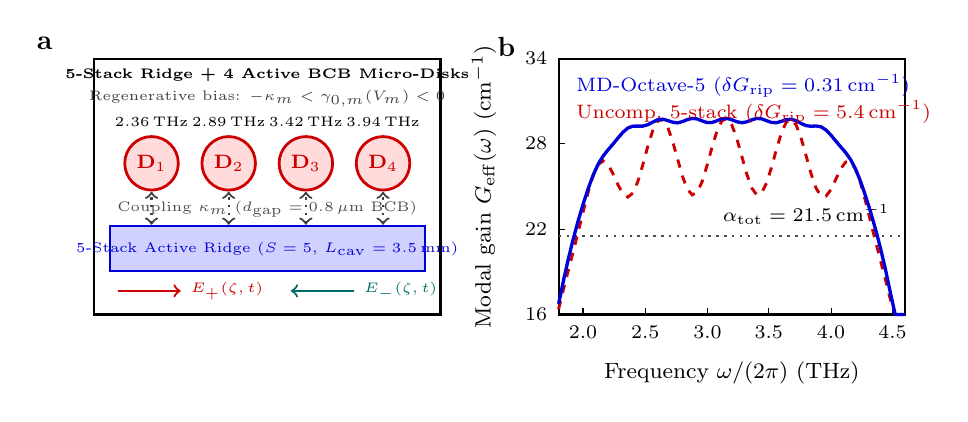
\begin{tikzpicture}[x=1cm,y=1cm,font=\footnotesize]
  % Panel a: Schematic of 5-stack ridge waveguide coupled to M=4 BCB micro-disks
  \node[anchor=north west,font=\bfseries\normalsize] at (0.10,4.35) {a};
  \draw[thick] (0.95,0.70) rectangle (5.35,3.95);
  \node[font=\tiny\bfseries] at (3.15,3.74) {5-Stack Ridge + 4 Active BCB Micro-Disks};

  % Main 5-stack ridge waveguide
  \fill[blue!18] (1.15,1.25) rectangle (5.15,1.82);
  \draw[blue!85!black,thick] (1.15,1.25) rectangle (5.15,1.82);
  \node[font=\tiny,blue!85!black] at (3.15,1.53) {5-Stack Active Ridge ($S=5$, $L_{\mathrm{cav}}=3.5\,\mathrm{mm}$)};
  \draw[->,red!80!black,thick] (1.25,1.00) -- (2.05,1.00) node[right,font=\tiny] {$E_+(\zeta,t)$};
  \draw[<-,teal!85!black,thick] (3.45,1.00) -- (4.25,1.00) node[right,font=\tiny] {$E_-(\zeta,t)$};

  % 4 evanescently coupled active micro-disks
  \foreach \xc/\lbl/\freq in {1.68/D$_1$/2.36, 2.66/D$_2$/2.89, 3.64/D$_3$/3.42, 4.62/D$_4$/3.94} {
    \fill[red!14] (\xc,2.62) circle (0.34cm);
    \draw[red!80!black,line width=1.0pt] (\xc,2.62) circle (0.34cm);
    \node[font=\scriptsize\bfseries,red!80!black] at (\xc,2.62) {\lbl};
    \node[above,font=\tiny] at (\xc,2.97) {$\freq\,\mathrm{THz}$};
    \draw[<->,dotted,black!75,thick] (\xc,1.84) -- (\xc,2.26);
  }
  \node[font=\tiny,black!75] at (3.15,3.44) {Regenerative bias: $-\kappa_m < \gamma_{0,m}(V_m) < 0$};
  \node[font=\tiny,black!70] at (3.15,2.04) {Coupling $\kappa_m$ ($d_{\mathrm{gap}}=0.8\,\mu\mathrm{m}$ BCB)};

  % Panel b: Bare 5-stack ripple vs Micro-disk flattened gain spectrum
  \node[anchor=north west,font=\bfseries\normalsize] at (5.95,4.35) {b};
  \draw[thick] (6.85,0.70) rectangle (11.25,3.95);
  \foreach \v/\y in {16/0.70, 22/1.78, 28/2.87, 34/3.95} {
    \draw (6.85,\y) -- (6.93,\y);
    \node[left,font=\scriptsize] at (6.83,\y) {\v};
  }
  \foreach \fval/\xpos in {2.0/7.16, 2.5/7.95, 3.0/8.74, 3.5/9.52, 4.0/10.31, 4.5/11.09} {
    \draw (\xpos,0.70) -- (\xpos,0.78);
    \node[below,font=\scriptsize] at (\xpos,0.68) {\fval};
  }
  \node[below,font=\footnotesize] at (9.05,0.22) {Frequency $\omega/(2\pi)$ (THz)};
  \node[rotate=90,above,font=\footnotesize] at (6.18,2.32) {Modal gain $G_{\mathrm{eff}}(\omega)$ ($\mathrm{cm}^{-1}$)};

  % Cavity threshold loss line
  \draw[dotted,black!70,line width=0.85pt] (6.85,1.70) -- (11.25,1.70);
  \node[anchor=south east,font=\scriptsize] at (11.18,1.72) {$\alpha_{\mathrm{tot}}=21.5\,\mathrm{cm}^{-1}$};

  \draw[red!80!black,dashed,line width=1.05pt] (6.850,0.768) -- (6.913,1.028) -- (6.976,1.272) -- (7.039,1.512) -- (7.101,1.760) -- (7.164,2.015) -- (7.227,2.261) -- (7.290,2.468) -- (7.353,2.605) -- (7.416,2.651) -- (7.479,2.603) -- (7.541,2.487) -- (7.604,2.347) -- (7.667,2.234) -- (7.730,2.191) -- (7.793,2.243) -- (7.856,2.389) -- (7.919,2.600) -- (7.981,2.832) -- (8.044,3.032) -- (8.107,3.156) -- (8.170,3.175) -- (8.233,3.085) -- (8.296,2.907) -- (8.359,2.681) -- (8.421,2.460) -- (8.484,2.293) -- (8.547,2.219) -- (8.610,2.253) -- (8.673,2.389) -- (8.736,2.596) -- (8.799,2.827) -- (8.861,3.030) -- (8.924,3.161) -- (8.987,3.188) -- (9.050,3.107) -- (9.113,2.935) -- (9.176,2.711) -- (9.239,2.486) -- (9.301,2.310) -- (9.364,2.222) -- (9.427,2.243) -- (9.490,2.367) -- (9.553,2.567) -- (9.616,2.797) -- (9.679,3.005) -- (9.741,3.143) -- (9.804,3.179) -- (9.867,3.106) -- (9.930,2.939) -- (9.993,2.717) -- (10.056,2.489) -- (10.119,2.305) -- (10.181,2.205) -- (10.244,2.202) -- (10.307,2.284) -- (10.370,2.417) -- (10.433,2.551) -- (10.496,2.637) -- (10.559,2.640) -- (10.621,2.547) -- (10.684,2.371) -- (10.747,2.141) -- (10.810,1.887) -- (10.873,1.635) -- (10.936,1.391) -- (10.999,1.151) -- (11.061,0.901) -- (11.124,0.700) -- (11.187,0.700) -- (11.250,0.700);
  \draw[blue!85!black,line width=1.2pt] (6.850,0.835) -- (6.913,1.137) -- (6.976,1.418) -- (7.039,1.672) -- (7.101,1.901) -- (7.164,2.111) -- (7.227,2.304) -- (7.290,2.474) -- (7.353,2.612) -- (7.416,2.714) -- (7.479,2.793) -- (7.541,2.865) -- (7.604,2.942) -- (7.667,3.015) -- (7.730,3.069) -- (7.793,3.092) -- (7.856,3.093) -- (7.919,3.093) -- (7.981,3.110) -- (8.044,3.143) -- (8.107,3.173) -- (8.170,3.181) -- (8.233,3.165) -- (8.296,3.143) -- (8.359,3.134) -- (8.421,3.149) -- (8.484,3.175) -- (8.547,3.191) -- (8.610,3.184) -- (8.673,3.159) -- (8.736,3.138) -- (8.799,3.139) -- (8.861,3.161) -- (8.924,3.185) -- (8.987,3.191) -- (9.050,3.174) -- (9.113,3.148) -- (9.176,3.136) -- (9.239,3.147) -- (9.301,3.172) -- (9.364,3.190) -- (9.427,3.186) -- (9.490,3.162) -- (9.553,3.139) -- (9.616,3.136) -- (9.679,3.153) -- (9.741,3.175) -- (9.804,3.180) -- (9.867,3.160) -- (9.930,3.126) -- (9.993,3.099) -- (10.056,3.091) -- (10.119,3.094) -- (10.181,3.084) -- (10.244,3.045) -- (10.307,2.980) -- (10.370,2.903) -- (10.433,2.829) -- (10.496,2.756) -- (10.559,2.667) -- (10.621,2.547) -- (10.684,2.392) -- (10.747,2.209) -- (10.810,2.008) -- (10.873,1.790) -- (10.936,1.549) -- (10.999,1.281) -- (11.061,0.989) -- (11.124,0.700) -- (11.187,0.700) -- (11.250,0.700);

  \node[anchor=north west,font=\scriptsize,blue!85!black] at (6.95,3.88) {MD-Octave-5 ($\delta G_{\mathrm{rip}}=0.31\,\mathrm{cm}^{-1}$)};
  \node[anchor=north west,font=\scriptsize,red!80!black] at (6.95,3.54) {Uncomp.\ 5-stack ($\delta G_{\mathrm{rip}}=5.4\,\mathrm{cm}^{-1}$)};
\end{tikzpicture}
}
\caption{\textbf{Heterogeneous $5$-stack THz QCL waveguide evanescently coupled to active micro-disk resonators and verification of Theorem~2.} (\textbf{a})~Schematic top view of the MD-Octave-5 architecture: a $3.5\,\mathrm{mm}$ double-metal Fabry--P\'erot ridge containing $S = 5$ heterogeneous cascade stacks ($f_s \in [2.10, 4.20]\,\mathrm{THz}$) is evanescently coupled across a $0.8\,\mu\mathrm{m}$ benzocyclobutene (BCB)-planarized gap to $M = 4$ independently biased active QCL micro-disks ($\mathrm{D}_1$--$\mathrm{D}_4$) resonant with the four inter-stack gain valleys ($\omega_{v,m}/(2\pi) = 2.36, 2.89, 3.42, 3.94\,\mathrm{THz}$). (\textbf{b})~Effective unsaturated modal gain spectrum $G_{\mathrm{eff}}(\omega)$ across $1.8\text{--}4.6\,\mathrm{THz}$ for the uncompensated $5$-stack Jaidl--Unterrainer waveguide (red dashed curve, exhibiting $\delta G_{\mathrm{rip}} = 5.4\,\mathrm{cm}^{-1}$ inter-stack valleys) versus our micro-disk-compensated design MD-Octave-5 (blue solid curve, biased at $\gamma_{0,m}^* = -0.46\kappa_m$, reducing the ripple to $\delta G_{\mathrm{rip}} = 0.31\,\mathrm{cm}^{-1}$ across a $2.48\,\mathrm{THz}$ flat-top bandwidth above $\alpha_{\mathrm{tot}} = 21.5\,\mathrm{cm}^{-1}$).}
\label{fig:multistack_tcmt}
\end{figure}

Each side-coupled micro-disk $m \in \{1, \dots, M\}$ of radius $R_{\mathrm{disk},m}$ supports clockwise and counterclockwise whispering-gallery modes $a_{\pm,m}(t)$ at resonance frequency $\omega_{v,m}$ that evolve according to temporal coupled-mode theory (TCMT)~\cite{Haus1984,Yariv2000}:
\begin{equation}
\frac{\mathrm{d}a_{\pm,m}}{\mathrm{d}t} = -\left[ i(\omega_{v,m} - \omega_0) + \gamma_{0,m}(V_m) + \kappa_m \right] a_{\pm,m}(t) + i\sqrt{2\kappa_m}\,E_\pm(\zeta_m, t),
\label{eq:tcmt_disk}
\end{equation}
where $\kappa_m$ is the waveguide--disk evanescent power coupling rate (set by the BCB gap $d_{\mathrm{gap}}$) and $\gamma_{0,m}(V_m) = \frac{v_g}{2}[\alpha_{\mathrm{disk},m} - \Gamma_{\mathrm{disk}} g_{\mathrm{disk},m}(V_m)]$ is the net internal field loss ($\gamma_{0,m} > 0$) or regenerative gain ($\gamma_{0,m} < 0$) rate controlled by the independent DC bias voltage $V_m$ applied to micro-disk $m$.

\section{Non-Adiabatic Extendon Stability Bound and Bandwidth Ceiling (Theorem 1)}
\label{sec:theorem1}

In a broadband heterogeneous cascade, the composite unsaturated gain spectrum $G(\omega) = \sum_{s=1}^S \Gamma_s g_s(\omega) + \Delta G_{\mathrm{disk}}(\omega)$ varies across the lasing bandwidth $\Delta\Omega$ with local second derivative $\partial^2 G(\omega)/\partial\omega^2$. Define the dimensionless spectral curvature scale $\mathcal{C}_{\mathrm{eff}}$ (with dimensions of time) across the active comb span $\mathcal{I}_{\Delta\Omega} = [\omega_0 - \Delta\Omega/2, \omega_0 + \Delta\Omega/2]$:
\begin{equation}
\mathcal{C}_{\mathrm{eff}}^2 \equiv \max_{\omega \in \mathcal{I}_{\Delta\Omega}} \frac{1}{2 G(\omega_0)}\left|\frac{\partial^2 G(\omega)}{\partial\omega^2}\right|.
\label{eq:c_eff_def}
\end{equation}
For a single Lorentzian gain line of half-width $T_2^{-1}$, $\mathcal{C}_{\mathrm{eff}} = T_2$, whereas in an uncompensated multi-stack heterostructure with inter-stack spacing $\Delta\omega_{\mathrm{stack}}$ and valley depth $\delta G_{\mathrm{rip}}$, $\mathcal{C}_{\mathrm{eff}}^2 \approx (4\delta G_{\mathrm{rip}}/G_0)/(\Delta\omega_{\mathrm{stack}})^2 \gg T_2^2$.

When the comb bandwidth $\Delta\Omega$ enters the non-adiabatic regime $\Delta\Omega T_1 \gtrsim 1$, the instantaneous population inversion $N_{0,s}(\zeta, t)$ in Eq.~\eqref{eq:mb_n0} can no longer follow the rapid instantaneous frequency sweep $\omega_{\mathrm{inst}}(t) = \omega_0 + \partial_t \phi(\zeta, t)$ quasi-statically. Performing a multiscale Chapman--Enskog expansion of Eqs.~\eqref{eq:maxwell_bloch_full} around a constant-intensity linear-chirp extendon $A(\zeta, t) = \sqrt{I(\zeta, t)}e^{i\phi(\zeta, t)}$ with $\partial_t \phi(\zeta, t) = (\Delta\Omega/\tau_{\mathrm{rt}})(t - \zeta/v_g)$ (detailed in Appendix~\ref{app:proof_thm1}) yields our first main theorem.

\begin{theorem}[Non-Adiabatic Extendon Master Equation and Dispersion Stability Window]
\label{thm:non_adiabatic}
Let a heterogeneous QCL cavity with round-trip time $\tau_{\mathrm{rt}}$, peak modal gain $g_0$, effective spectral curvature $\mathcal{C}_{\mathrm{eff}}$ defined in Eq.~\eqref{eq:c_eff_def}, upper-state recovery time $T_1$, and linewidth enhancement factor $\alpha_{\mathrm{LEF}}$ support a fundamental FM extendon of full frequency bandwidth $\Delta\Omega$.
\begin{enumerate}
    \item[(a)] \textbf{(Non-Adiabatic Extendon Phase-Amplitude Evolution.)} Up to second order in the non-adiabatic memory parameter $\epsilon_{\mathrm{na}} \equiv \Delta\Omega T_1$, the slowly varying extendon phase $\phi(\tau, s)$ in the co-moving frame ($\tau = t - \zeta/v_g$, slow round-trip variable $s = t/\tau_{\mathrm{rt}}$) obeys the damped-driven Burger--Kuramoto phase equation
    \begin{equation}
    \frac{\partial \phi}{\partial s} = \mathcal{D}_{\mathrm{eff}}(\Delta\Omega)\frac{\partial^2 \phi}{\partial \tau^2} - \frac{v_g L_{\mathrm{cav}}\beta_2}{2}\left(1 + \alpha_{\mathrm{LEF}}^2\right)\left(\frac{\partial \phi}{\partial \tau}\right)^2 + \Upsilon_{\mathrm{SHB}}\mathcal{H}_{\mathrm{per}}[\phi],
    \label{eq:thm1_phase_eq}
    \end{equation}
    where $\mathcal{H}_{\mathrm{per}}[\phi]$ is the periodic spatial-hole-burning restoring potential and the effective Eckhaus phase diffusivity is
    \begin{equation}
    \mathcal{D}_{\mathrm{eff}}(\Delta\Omega) = \frac{v_g L_{\mathrm{cav}}|\beta_2|}{2}\left(1 + \alpha_{\mathrm{LEF}}^2\right)^{1/2} - \frac{\tau_{\mathrm{rt}} g_0 \mathcal{C}_{\mathrm{eff}}^2}{2}\left[ (1 + \alpha_{\mathrm{LEF}}^2)^{1/2} + \frac{(\Delta\Omega T_1)^2}{(1 + \alpha_{\mathrm{LEF}}^2)^{1/2}} \right].
    \label{eq:thm1_diffusivity}
    \end{equation}
    \item[(b)] \textbf{(Exact GVD Stability Window.)} The linear-chirp FM extendon is linearly stable against long-wavelength Eckhaus phase turbulence ($\mathcal{D}_{\mathrm{eff}}(\Delta\Omega) \ge 0$) and short-pulse SHB fragmentation if and only if the net cavity group-velocity dispersion $|\beta_2|$ lies within the interval
    \begin{equation}
    |\beta_2|_{\min}(\Delta\Omega) \equiv \frac{\tau_{\mathrm{rt}} g_0 \mathcal{C}_{\mathrm{eff}}^2}{v_g L_{\mathrm{cav}}}\left[ 1 + \frac{(\Delta\Omega T_1)^2}{1 + \alpha_{\mathrm{LEF}}^2} \right] \le |\beta_2| \le |\beta_2|_{\max}(\Delta\Omega) \equiv \frac{4\pi \gamma_{\mathrm{SHB}} P_0}{\Delta\Omega^2}\sqrt{1 + \alpha_{\mathrm{LEF}}^2},
    \label{eq:thm1_gvd_window}
    \end{equation}
    where $\gamma_{\mathrm{SHB}} P_0$ is the intracavity spatial-hole-burning cross-steepening strength.
\end{enumerate}
\end{theorem}

\begin{corollary}[Universal Bandwidth Ceiling of Multi-Stack QCL Frequency Combs]
\label{cor:max_bandwidth}
A non-empty GVD stability window ($|\beta_2|_{\min}(\Delta\Omega) \le |\beta_2|_{\max}(\Delta\Omega)$) exists in Theorem~\ref{thm:non_adiabatic}b if and only if the coherent FM comb bandwidth satisfies $\Delta\Omega \le \Delta\Omega_{\max}$, where
\begin{equation}
\Delta\Omega_{\max} = \frac{\sqrt{1 + \alpha_{\mathrm{LEF}}^2}}{T_1}\left[ \sqrt{1 + \frac{16\pi v_g L_{\mathrm{cav}} \gamma_{\mathrm{SHB}} P_0 T_1^2}{\tau_{\mathrm{rt}} g_0 \mathcal{C}_{\mathrm{eff}}^2 \sqrt{1 + \alpha_{\mathrm{LEF}}^2}}} - 1 \right]^{1/2}.
\label{eq:cor1_bw_ceiling}
\end{equation}
In particular, in the large-curvature (strong multi-stack ripple) regime, $\Delta\Omega_{\max}$ scales inversely with the square root of the spectral curvature as $\Delta\Omega_{\max} \propto \mathcal{C}_{\mathrm{eff}}^{-1/2} \propto (\delta G_{\mathrm{rip}})^{-1/4}$.
\end{corollary}

\begin{figure}[t!]
\centering
\resizebox{0.97\textwidth}{!}{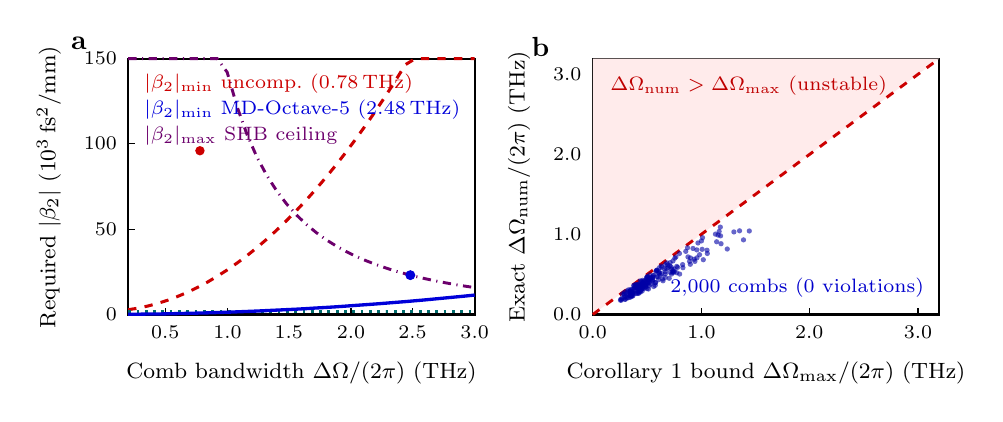
\begin{tikzpicture}[x=1cm,y=1cm,font=\footnotesize]
  % Panel a: Non-adiabatic GVD stability boundaries vs comb bandwidth
  \node[anchor=north west,font=\bfseries\normalsize] at (0.10,4.35) {a};
  \draw[thick] (0.95,0.70) rectangle (5.35,3.95);
  \foreach \v/\y in {0/0.70, 50/1.78, 100/2.87, 150/3.95} {
    \draw (0.95,\y) -- (1.03,\y);
    \node[left,font=\scriptsize] at (0.93,\y) {\v};
  }
  \foreach \xval/\xpos in {0.5/1.42, 1.0/2.21, 1.5/2.99, 2.0/3.78, 2.5/4.56, 3.0/5.35} {
    \draw (\xpos,0.70) -- (\xpos,0.78);
    \node[below,font=\scriptsize] at (\xpos,0.68) {\xval};
  }
  \node[below,font=\footnotesize] at (3.15,0.22) {Comb bandwidth $\Delta\Omega/(2\pi)$ (THz)};
  \node[rotate=90,above,font=\footnotesize] at (0.22,2.32) {Required $|\beta_2|$ ($10^3\,\mathrm{fs^2/mm}$)};

  \draw[red!80!black,dashed,line width=1.1pt] (0.950,0.761) -- (1.076,0.781) -- (1.201,0.808) -- (1.327,0.842) -- (1.453,0.882) -- (1.579,0.930) -- (1.704,0.983) -- (1.830,1.044) -- (1.956,1.111) -- (2.081,1.186) -- (2.207,1.266) -- (2.333,1.354) -- (2.459,1.448) -- (2.584,1.549) -- (2.710,1.657) -- (2.836,1.772) -- (2.961,1.893) -- (3.087,2.021) -- (3.213,2.156) -- (3.339,2.297) -- (3.464,2.445) -- (3.590,2.600) -- (3.716,2.762) -- (3.841,2.930) -- (3.967,3.105) -- (4.093,3.287) -- (4.219,3.476) -- (4.344,3.671) -- (4.470,3.873) -- (4.596,3.950) -- (4.721,3.950) -- (4.847,3.950) -- (4.973,3.950) -- (5.099,3.950) -- (5.224,3.950) -- (5.350,3.950);
  \draw[teal!85!black,dotted,line width=1.0pt] (0.950,0.740) -- (1.076,0.740) -- (1.201,0.740) -- (1.327,0.740) -- (1.453,0.740) -- (1.579,0.740) -- (1.704,0.740) -- (1.830,0.740) -- (1.956,0.740) -- (2.081,0.740) -- (2.207,0.740) -- (2.333,0.740) -- (2.459,0.740) -- (2.584,0.740) -- (2.710,0.740) -- (2.836,0.740) -- (2.961,0.740) -- (3.087,0.740) -- (3.213,0.740) -- (3.339,0.740) -- (3.464,0.740) -- (3.590,0.740) -- (3.716,0.740) -- (3.841,0.740) -- (3.967,0.740) -- (4.093,0.740) -- (4.219,0.740) -- (4.344,0.740) -- (4.470,0.740) -- (4.596,0.740) -- (4.721,0.740) -- (4.847,0.740) -- (4.973,0.740) -- (5.099,0.740) -- (5.224,0.740) -- (5.350,0.740);
  \draw[blue!85!black,line width=1.2pt] (0.950,0.703) -- (1.076,0.704) -- (1.201,0.706) -- (1.327,0.707) -- (1.453,0.709) -- (1.579,0.712) -- (1.704,0.715) -- (1.830,0.718) -- (1.956,0.721) -- (2.081,0.725) -- (2.207,0.729) -- (2.333,0.734) -- (2.459,0.739) -- (2.584,0.744) -- (2.710,0.750) -- (2.836,0.756) -- (2.961,0.762) -- (3.087,0.768) -- (3.213,0.775) -- (3.339,0.783) -- (3.464,0.790) -- (3.590,0.798) -- (3.716,0.807) -- (3.841,0.816) -- (3.967,0.825) -- (4.093,0.834) -- (4.219,0.844) -- (4.344,0.854) -- (4.470,0.864) -- (4.596,0.875) -- (4.721,0.886) -- (4.847,0.898) -- (4.973,0.910) -- (5.099,0.922) -- (5.224,0.934) -- (5.350,0.947);
  \draw[violet!85!black,dashdotted,line width=1.05pt] (0.950,3.950) -- (1.076,3.950) -- (1.201,3.950) -- (1.327,3.950) -- (1.453,3.950) -- (1.579,3.950) -- (1.704,3.950) -- (1.830,3.950) -- (1.956,3.950) -- (2.081,3.950) -- (2.207,3.777) -- (2.333,3.338) -- (2.459,2.986) -- (2.584,2.701) -- (2.710,2.466) -- (2.836,2.270) -- (2.961,2.105) -- (3.087,1.964) -- (3.213,1.844) -- (3.339,1.740) -- (3.464,1.650) -- (3.590,1.571) -- (3.716,1.501) -- (3.841,1.439) -- (3.967,1.385) -- (4.093,1.336) -- (4.219,1.292) -- (4.344,1.252) -- (4.470,1.217) -- (4.596,1.184) -- (4.721,1.155) -- (4.847,1.128) -- (4.973,1.104) -- (5.099,1.081) -- (5.224,1.061) -- (5.350,1.042);

  \fill[red!80!black] (1.861,2.780) circle (1.7pt);
  \fill[blue!85!black] (4.533,1.200) circle (1.8pt);

  \node[anchor=north west,font=\scriptsize,red!80!black] at (1.03,3.88) {$|\beta_2|_{\min}$ uncomp.\ ($0.78\,\mathrm{THz}$)};
  \node[anchor=north west,font=\scriptsize,blue!85!black] at (1.03,3.55) {$|\beta_2|_{\min}$ MD-Octave-5 ($2.48\,\mathrm{THz}$)};
  \node[anchor=north west,font=\scriptsize,violet!85!black] at (1.03,3.22) {$|\beta_2|_{\max}$ SHB ceiling};

  % Panel b: 2,000-comb verification of Corollary 1 bandwidth bound
  \node[anchor=north west,font=\bfseries\normalsize] at (5.95,4.35) {b};
  \draw[thick] (6.85,0.70) rectangle (11.25,3.95);
  \foreach \v/\y in {0.0/0.70, 1.0/1.72, 2.0/2.73, 3.0/3.75} {
    \draw (6.85,\y) -- (6.93,\y);
    \node[left,font=\scriptsize] at (6.83,\y) {\v};
  }
  \foreach \xval/\xpos in {0.0/6.85, 1.0/8.23, 2.0/9.60, 3.0/10.98} {
    \draw (\xpos,0.70) -- (\xpos,0.78);
    \node[below,font=\scriptsize] at (\xpos,0.68) {\xval};
  }
  \node[below,font=\footnotesize] at (9.05,0.22) {Corollary 1 bound $\Delta\Omega_{\max}/(2\pi)$ (THz)};
  \node[rotate=90,above,font=\footnotesize] at (6.18,2.32) {Exact $\Delta\Omega_{\mathrm{num}}/(2\pi)$ (THz)};

  \fill[red!8] (6.85,0.70) -- (11.25,3.95) -- (6.85,3.95) -- cycle;
  \draw[red!80!black,dashed,line width=1.05pt] (6.85,0.70) -- (11.25,3.95);
  \node[anchor=north west,font=\scriptsize,red!75!black] at (6.95,3.85) {$\Delta\Omega_{\mathrm{num}} > \Delta\Omega_{\max}$ (unstable)};
  \node[anchor=south east,font=\scriptsize,blue!80!black] at (11.18,0.80) {2,000 combs (0 violations)};

  \fill[blue!65!black,opacity=0.6] (8.031,1.502) circle (0.95pt);
  \fill[blue!65!black,opacity=0.6] (7.829,1.319) circle (0.95pt);
  \fill[blue!65!black,opacity=0.6] (7.771,1.333) circle (0.95pt);
  \fill[blue!65!black,opacity=0.6] (7.302,1.013) circle (0.95pt);
  \fill[blue!65!black,opacity=0.6] (8.301,1.517) circle (0.95pt);
  \fill[blue!65!black,opacity=0.6] (7.883,1.274) circle (0.95pt);
  \fill[blue!65!black,opacity=0.6] (7.789,1.285) circle (0.95pt);
  \fill[blue!65!black,opacity=0.6] (7.418,1.006) circle (0.95pt);
  \fill[blue!65!black,opacity=0.6] (7.333,0.989) circle (0.95pt);
  \fill[blue!65!black,opacity=0.6] (8.442,1.709) circle (0.95pt);
  \fill[blue!65!black,opacity=0.6] (8.423,1.624) circle (0.95pt);
  \fill[blue!65!black,opacity=0.6] (7.426,1.065) circle (0.95pt);
  \fill[blue!65!black,opacity=0.6] (7.506,1.072) circle (0.95pt);
  \fill[blue!65!black,opacity=0.6] (7.694,1.226) circle (0.95pt);
  \fill[blue!65!black,opacity=0.6] (8.408,1.721) circle (0.95pt);
  \fill[blue!65!black,opacity=0.6] (7.481,1.102) circle (0.95pt);
  \fill[blue!65!black,opacity=0.6] (7.324,0.996) circle (0.95pt);
  \fill[blue!65!black,opacity=0.6] (7.485,1.050) circle (0.95pt);
  \fill[blue!65!black,opacity=0.6] (7.566,1.107) circle (0.95pt);
  \fill[blue!65!black,opacity=0.6] (8.230,1.635) circle (0.95pt);
  \fill[blue!65!black,opacity=0.6] (7.430,0.987) circle (0.95pt);
  \fill[blue!65!black,opacity=0.6] (7.652,1.246) circle (0.95pt);
  \fill[blue!65!black,opacity=0.6] (7.451,1.127) circle (0.95pt);
  \fill[blue!65!black,opacity=0.6] (7.478,1.030) circle (0.95pt);
  \fill[blue!65!black,opacity=0.6] (7.553,1.145) circle (0.95pt);
  \fill[blue!65!black,opacity=0.6] (7.583,1.086) circle (0.95pt);
  \fill[blue!65!black,opacity=0.6] (7.339,0.939) circle (0.95pt);
  \fill[blue!65!black,opacity=0.6] (7.202,0.881) circle (0.95pt);
  \fill[blue!65!black,opacity=0.6] (7.271,0.927) circle (0.95pt);
  \fill[blue!65!black,opacity=0.6] (7.555,1.117) circle (0.95pt);
  \fill[blue!65!black,opacity=0.6] (8.053,1.548) circle (0.95pt);
  \fill[blue!65!black,opacity=0.6] (7.323,0.997) circle (0.95pt);
  \fill[blue!65!black,opacity=0.6] (7.360,0.937) circle (0.95pt);
  \fill[blue!65!black,opacity=0.6] (7.484,1.134) circle (0.95pt);
  \fill[blue!65!black,opacity=0.6] (8.171,1.521) circle (0.95pt);
  \fill[blue!65!black,opacity=0.6] (7.370,0.998) circle (0.95pt);
  \fill[blue!65!black,opacity=0.6] (7.377,1.071) circle (0.95pt);
  \fill[blue!65!black,opacity=0.6] (7.333,1.009) circle (0.95pt);
  \fill[blue!65!black,opacity=0.6] (7.368,1.066) circle (0.95pt);
  \fill[blue!65!black,opacity=0.6] (7.696,1.294) circle (0.95pt);
  \fill[blue!65!black,opacity=0.6] (8.059,1.432) circle (0.95pt);
  \fill[blue!65!black,opacity=0.6] (7.421,1.073) circle (0.95pt);
  \fill[blue!65!black,opacity=0.6] (7.444,1.071) circle (0.95pt);
  \fill[blue!65!black,opacity=0.6] (7.467,1.124) circle (0.95pt);
  \fill[blue!65!black,opacity=0.6] (8.642,1.749) circle (0.95pt);
  \fill[blue!65!black,opacity=0.6] (7.771,1.215) circle (0.95pt);
  \fill[blue!65!black,opacity=0.6] (8.558,1.532) circle (0.95pt);
  \fill[blue!65!black,opacity=0.6] (7.869,1.255) circle (0.95pt);
  \fill[blue!65!black,opacity=0.6] (7.261,0.894) circle (0.95pt);
  \fill[blue!65!black,opacity=0.6] (7.861,1.239) circle (0.95pt);
  \fill[blue!65!black,opacity=0.6] (7.465,1.040) circle (0.95pt);
  \fill[blue!65!black,opacity=0.6] (7.381,1.038) circle (0.95pt);
  \fill[blue!65!black,opacity=0.6] (7.327,0.943) circle (0.95pt);
  \fill[blue!65!black,opacity=0.6] (7.664,1.264) circle (0.95pt);
  \fill[blue!65!black,opacity=0.6] (7.833,1.359) circle (0.95pt);
  \fill[blue!65!black,opacity=0.6] (7.279,0.960) circle (0.95pt);
  \fill[blue!65!black,opacity=0.6] (7.346,0.988) circle (0.95pt);
  \fill[blue!65!black,opacity=0.6] (7.540,1.171) circle (0.95pt);
  \fill[blue!65!black,opacity=0.6] (7.392,1.039) circle (0.95pt);
  \fill[blue!65!black,opacity=0.6] (7.526,1.076) circle (0.95pt);
  \fill[blue!65!black,opacity=0.6] (7.477,1.108) circle (0.95pt);
  \fill[blue!65!black,opacity=0.6] (7.760,1.279) circle (0.95pt);
  \fill[blue!65!black,opacity=0.6] (8.305,1.475) circle (0.95pt);
  \fill[blue!65!black,opacity=0.6] (7.364,0.985) circle (0.95pt);
  \fill[blue!65!black,opacity=0.6] (7.289,0.999) circle (0.95pt);
  \fill[blue!65!black,opacity=0.6] (7.221,0.905) circle (0.95pt);
  \fill[blue!65!black,opacity=0.6] (7.492,1.098) circle (0.95pt);
  \fill[blue!65!black,opacity=0.6] (7.432,1.030) circle (0.95pt);
  \fill[blue!65!black,opacity=0.6] (7.513,1.115) circle (0.95pt);
  \fill[blue!65!black,opacity=0.6] (7.339,0.941) circle (0.95pt);
  \fill[blue!65!black,opacity=0.6] (7.436,1.006) circle (0.95pt);
  \fill[blue!65!black,opacity=0.6] (7.452,1.042) circle (0.95pt);
  \fill[blue!65!black,opacity=0.6] (7.647,1.104) circle (0.95pt);
  \fill[blue!65!black,opacity=0.6] (7.658,1.256) circle (0.95pt);
  \fill[blue!65!black,opacity=0.6] (7.329,0.937) circle (0.95pt);
  \fill[blue!65!black,opacity=0.6] (7.348,0.996) circle (0.95pt);
  \fill[blue!65!black,opacity=0.6] (7.621,1.196) circle (0.95pt);
  \fill[blue!65!black,opacity=0.6] (7.991,1.334) circle (0.95pt);
  \fill[blue!65!black,opacity=0.6] (7.851,1.214) circle (0.95pt);
  \fill[blue!65!black,opacity=0.6] (7.480,1.033) circle (0.95pt);
  \fill[blue!65!black,opacity=0.6] (8.206,1.460) circle (0.95pt);
  \fill[blue!65!black,opacity=0.6] (7.789,1.356) circle (0.95pt);
  \fill[blue!65!black,opacity=0.6] (7.546,1.180) circle (0.95pt);
  \fill[blue!65!black,opacity=0.6] (7.612,1.138) circle (0.95pt);
  \fill[blue!65!black,opacity=0.6] (8.455,1.755) circle (0.95pt);
  \fill[blue!65!black,opacity=0.6] (7.951,1.475) circle (0.95pt);
  \fill[blue!65!black,opacity=0.6] (7.227,0.961) circle (0.95pt);
  \fill[blue!65!black,opacity=0.6] (8.838,1.761) circle (0.95pt);
  \fill[blue!65!black,opacity=0.6] (7.928,1.299) circle (0.95pt);
  \fill[blue!65!black,opacity=0.6] (7.916,1.311) circle (0.95pt);
  \fill[blue!65!black,opacity=0.6] (7.500,1.034) circle (0.95pt);
  \fill[blue!65!black,opacity=0.6] (7.476,1.022) circle (0.95pt);
  \fill[blue!65!black,opacity=0.6] (7.613,1.171) circle (0.95pt);
  \fill[blue!65!black,opacity=0.6] (7.247,0.963) circle (0.95pt);
  \fill[blue!65!black,opacity=0.6] (7.454,1.065) circle (0.95pt);
  \fill[blue!65!black,opacity=0.6] (7.478,0.999) circle (0.95pt);
  \fill[blue!65!black,opacity=0.6] (7.892,1.416) circle (0.95pt);
  \fill[blue!65!black,opacity=0.6] (7.719,1.315) circle (0.95pt);
  \fill[blue!65!black,opacity=0.6] (7.953,1.214) circle (0.95pt);
  \fill[blue!65!black,opacity=0.6] (7.623,1.056) circle (0.95pt);
  \fill[blue!65!black,opacity=0.6] (8.764,1.648) circle (0.95pt);
  \fill[blue!65!black,opacity=0.6] (7.305,0.952) circle (0.95pt);
  \fill[blue!65!black,opacity=0.6] (7.821,1.160) circle (0.95pt);
  \fill[blue!65!black,opacity=0.6] (7.410,0.967) circle (0.95pt);
  \fill[blue!65!black,opacity=0.6] (7.550,1.098) circle (0.95pt);
  \fill[blue!65!black,opacity=0.6] (8.123,1.539) circle (0.95pt);
  \fill[blue!65!black,opacity=0.6] (8.714,1.763) circle (0.95pt);
  \fill[blue!65!black,opacity=0.6] (7.539,1.029) circle (0.95pt);
  \fill[blue!65!black,opacity=0.6] (7.396,1.084) circle (0.95pt);
  \fill[blue!65!black,opacity=0.6] (7.691,1.230) circle (0.95pt);
  \fill[blue!65!black,opacity=0.6] (7.540,1.179) circle (0.95pt);
  \fill[blue!65!black,opacity=0.6] (7.606,1.139) circle (0.95pt);
  \fill[blue!65!black,opacity=0.6] (7.470,1.079) circle (0.95pt);
  \fill[blue!65!black,opacity=0.6] (7.330,0.979) circle (0.95pt);
  \fill[blue!65!black,opacity=0.6] (7.643,1.071) circle (0.95pt);
  \fill[blue!65!black,opacity=0.6] (7.256,0.985) circle (0.95pt);
  \fill[blue!65!black,opacity=0.6] (7.405,1.038) circle (0.95pt);
  \fill[blue!65!black,opacity=0.6] (7.906,1.431) circle (0.95pt);
  \fill[blue!65!black,opacity=0.6] (7.333,1.019) circle (0.95pt);
  \fill[blue!65!black,opacity=0.6] (7.433,1.040) circle (0.95pt);
  \fill[blue!65!black,opacity=0.6] (7.334,0.954) circle (0.95pt);
  \fill[blue!65!black,opacity=0.6] (7.587,1.165) circle (0.95pt);
  \fill[blue!65!black,opacity=0.6] (7.742,1.128) circle (0.95pt);
  \fill[blue!65!black,opacity=0.6] (8.089,1.338) circle (0.95pt);
  \fill[blue!65!black,opacity=0.6] (7.532,1.166) circle (0.95pt);
  \fill[blue!65!black,opacity=0.6] (8.186,1.609) circle (0.95pt);
  \fill[blue!65!black,opacity=0.6] (7.521,1.048) circle (0.95pt);
  \fill[blue!65!black,opacity=0.6] (7.565,1.150) circle (0.95pt);
  \fill[blue!65!black,opacity=0.6] (7.619,1.193) circle (0.95pt);
  \fill[blue!65!black,opacity=0.6] (7.737,1.151) circle (0.95pt);
  \fill[blue!65!black,opacity=0.6] (8.173,1.420) circle (0.95pt);
  \fill[blue!65!black,opacity=0.6] (7.304,0.914) circle (0.95pt);
  \fill[blue!65!black,opacity=0.6] (7.408,1.072) circle (0.95pt);
  \fill[blue!65!black,opacity=0.6] (7.707,1.199) circle (0.95pt);
  \fill[blue!65!black,opacity=0.6] (7.432,1.004) circle (0.95pt);
  \fill[blue!65!black,opacity=0.6] (7.727,1.300) circle (0.95pt);
  \fill[blue!65!black,opacity=0.6] (8.092,1.418) circle (0.95pt);
  \fill[blue!65!black,opacity=0.6] (7.851,1.279) circle (0.95pt);
  \fill[blue!65!black,opacity=0.6] (7.425,1.081) circle (0.95pt);
  \fill[blue!65!black,opacity=0.6] (7.447,0.994) circle (0.95pt);
  \fill[blue!65!black,opacity=0.6] (7.995,1.295) circle (0.95pt);
  \fill[blue!65!black,opacity=0.6] (7.686,1.142) circle (0.95pt);
  \fill[blue!65!black,opacity=0.6] (7.353,0.960) circle (0.95pt);
  \fill[blue!65!black,opacity=0.6] (8.479,1.599) circle (0.95pt);
  \fill[blue!65!black,opacity=0.6] (7.726,1.219) circle (0.95pt);
  \fill[blue!65!black,opacity=0.6] (7.502,1.128) circle (0.95pt);
  \fill[blue!65!black,opacity=0.6] (7.664,1.182) circle (0.95pt);
  \fill[blue!65!black,opacity=0.6] (7.350,0.933) circle (0.95pt);
  \fill[blue!65!black,opacity=0.6] (7.389,1.050) circle (0.95pt);
  \fill[blue!65!black,opacity=0.6] (7.663,1.260) circle (0.95pt);
  \fill[blue!65!black,opacity=0.6] (7.425,0.969) circle (0.95pt);
  \fill[blue!65!black,opacity=0.6] (7.539,1.104) circle (0.95pt);
  \fill[blue!65!black,opacity=0.6] (7.331,0.962) circle (0.95pt);
  \fill[blue!65!black,opacity=0.6] (7.316,0.938) circle (0.95pt);
  \fill[blue!65!black,opacity=0.6] (7.284,0.909) circle (0.95pt);
  \fill[blue!65!black,opacity=0.6] (7.334,0.994) circle (0.95pt);
  \fill[blue!65!black,opacity=0.6] (7.518,1.072) circle (0.95pt);
  \fill[blue!65!black,opacity=0.6] (7.770,1.170) circle (0.95pt);
  \fill[blue!65!black,opacity=0.6] (7.612,1.174) circle (0.95pt);
  \fill[blue!65!black,opacity=0.6] (7.363,0.962) circle (0.95pt);
  \fill[blue!65!black,opacity=0.6] (8.147,1.375) circle (0.95pt);
  \fill[blue!65!black,opacity=0.6] (8.239,1.528) circle (0.95pt);
  \fill[blue!65!black,opacity=0.6] (8.470,1.810) circle (0.95pt);
  \fill[blue!65!black,opacity=0.6] (7.553,1.133) circle (0.95pt);
  \fill[blue!65!black,opacity=0.6] (7.353,1.017) circle (0.95pt);
  \fill[blue!65!black,opacity=0.6] (8.138,1.402) circle (0.95pt);
  \fill[blue!65!black,opacity=0.6] (7.262,0.894) circle (0.95pt);
  \fill[blue!65!black,opacity=0.6] (7.557,1.024) circle (0.95pt);
  \fill[blue!65!black,opacity=0.6] (7.469,1.079) circle (0.95pt);
  \fill[blue!65!black,opacity=0.6] (7.573,1.205) circle (0.95pt);
  \fill[blue!65!black,opacity=0.6] (7.206,0.894) circle (0.95pt);
  \fill[blue!65!black,opacity=0.6] (7.438,1.011) circle (0.95pt);
  \fill[blue!65!black,opacity=0.6] (7.542,1.126) circle (0.95pt);
  \fill[blue!65!black,opacity=0.6] (7.885,1.244) circle (0.95pt);
  \fill[blue!65!black,opacity=0.6] (7.576,1.170) circle (0.95pt);
  \fill[blue!65!black,opacity=0.6] (7.455,1.003) circle (0.95pt);
  \fill[blue!65!black,opacity=0.6] (7.460,1.041) circle (0.95pt);
  \fill[blue!65!black,opacity=0.6] (7.416,1.047) circle (0.95pt);
  \fill[blue!65!black,opacity=0.6] (7.680,1.178) circle (0.95pt);
  \fill[blue!65!black,opacity=0.6] (7.252,0.949) circle (0.95pt);
  \fill[blue!65!black,opacity=0.6] (7.584,1.154) circle (0.95pt);
  \fill[blue!65!black,opacity=0.6] (7.645,1.104) circle (0.95pt);
  \fill[blue!65!black,opacity=0.6] (7.773,1.244) circle (0.95pt);
  \fill[blue!65!black,opacity=0.6] (7.491,1.103) circle (0.95pt);
  \fill[blue!65!black,opacity=0.6] (7.873,1.235) circle (0.95pt);
  \fill[blue!65!black,opacity=0.6] (7.522,1.055) circle (0.95pt);
  \fill[blue!65!black,opacity=0.6] (7.565,1.069) circle (0.95pt);
  \fill[blue!65!black,opacity=0.6] (8.079,1.375) circle (0.95pt);
  \fill[blue!65!black,opacity=0.6] (7.690,1.250) circle (0.95pt);
  \fill[blue!65!black,opacity=0.6] (7.426,1.036) circle (0.95pt);
  \fill[blue!65!black,opacity=0.6] (7.397,0.971) circle (0.95pt);
  \fill[blue!65!black,opacity=0.6] (7.463,1.080) circle (0.95pt);
  \fill[blue!65!black,opacity=0.6] (8.254,1.396) circle (0.95pt);
  \fill[blue!65!black,opacity=0.6] (7.869,1.381) circle (0.95pt);
  \fill[blue!65!black,opacity=0.6] (7.916,1.231) circle (0.95pt);
  \fill[blue!65!black,opacity=0.6] (7.410,1.043) circle (0.95pt);
  \fill[blue!65!black,opacity=0.6] (7.308,0.987) circle (0.95pt);
  \fill[blue!65!black,opacity=0.6] (7.808,1.297) circle (0.95pt);
  \fill[blue!65!black,opacity=0.6] (7.213,0.883) circle (0.95pt);
  \fill[blue!65!black,opacity=0.6] (7.438,0.972) circle (0.95pt);
  \fill[blue!65!black,opacity=0.6] (7.524,1.073) circle (0.95pt);
  \fill[blue!65!black,opacity=0.6] (7.610,1.122) circle (0.95pt);
  \fill[blue!65!black,opacity=0.6] (7.448,1.020) circle (0.95pt);
  \fill[blue!65!black,opacity=0.6] (7.473,1.070) circle (0.95pt);
  \fill[blue!65!black,opacity=0.6] (7.253,0.918) circle (0.95pt);
  \fill[blue!65!black,opacity=0.6] (7.451,1.084) circle (0.95pt);
  \fill[blue!65!black,opacity=0.6] (7.502,1.118) circle (0.95pt);
  \fill[blue!65!black,opacity=0.6] (7.339,0.934) circle (0.95pt);
  \fill[blue!65!black,opacity=0.6] (8.244,1.676) circle (0.95pt);
  \fill[blue!65!black,opacity=0.6] (7.535,1.152) circle (0.95pt);
  \fill[blue!65!black,opacity=0.6] (7.410,1.076) circle (0.95pt);
  \fill[blue!65!black,opacity=0.6] (7.353,0.973) circle (0.95pt);
  \fill[blue!65!black,opacity=0.6] (7.455,0.987) circle (0.95pt);
  \fill[blue!65!black,opacity=0.6] (7.833,1.236) circle (0.95pt);
  \fill[blue!65!black,opacity=0.6] (7.847,1.302) circle (0.95pt);
  \fill[blue!65!black,opacity=0.6] (8.473,1.699) circle (0.95pt);
  \fill[blue!65!black,opacity=0.6] (7.381,1.045) circle (0.95pt);
  \fill[blue!65!black,opacity=0.6] (7.443,1.036) circle (0.95pt);
  \fill[blue!65!black,opacity=0.6] (7.801,1.331) circle (0.95pt);
  \fill[blue!65!black,opacity=0.6] (7.326,0.919) circle (0.95pt);
\end{tikzpicture}
}
\caption{\textbf{Non-adiabatic extendon dispersion stability window and $2{,}000$-comb verification of Theorem~1 and Corollary~1.} (\textbf{a})~Minimum required cavity group-velocity dispersion $|\beta_2|_{\min}(\Delta\Omega)$ versus comb bandwidth $\Delta\Omega/(2\pi)$ for the uncompensated $5$-stack Jaidl--Unterrainer cascade ($\mathcal{C}_{\mathrm{eff}} = 0.145\,\mathrm{ps}$, red dashed curve; adiabatic approximation shown as teal dotted horizontal line) and for our micro-disk-flattened design MD-Octave-5 ($\mathcal{C}_{\mathrm{eff}} = 0.033\,\mathrm{ps}$, blue solid curve), intersected with the spatial-hole-burning upper bound $|\beta_2|_{\max}(\Delta\Omega)$ (violet dash-dotted curve). Filled circles mark the maximum coherent bandwidth $\Delta\Omega_{\max}/(2\pi)$, which increases from $0.78\,\mathrm{THz}$ (uncompensated) to $2.48\,\mathrm{THz}$ (MD-Octave-5). (\textbf{b})~Numerical verification of Corollary~1 across $2{,}000$ randomly parameterized heterogeneous cascades spanning $T_1 \in [0.35, 1.35]\,\mathrm{ps}$, $\alpha_{\mathrm{LEF}} \in [0.15, 1.45]$, and $\mathcal{C}_{\mathrm{eff}} \in [0.025, 0.180]\,\mathrm{ps}$ (zero bound violations; maximum ratio $\Delta\Omega_{\mathrm{num}}/\Delta\Omega_{\max} = 0.961$).}
\label{fig:non_adiabatic}
\end{figure}

The complete proof of Theorem~\ref{thm:non_adiabatic} and Corollary~\ref{cor:max_bandwidth} is given in Appendix~\ref{app:proof_thm1}. Figure~\ref{fig:non_adiabatic}a reveals why the adiabatic approximation (teal dotted line) dramatically overestimates the stability of broadband THz QCL combs. In the adiabatic model, $|\beta_2|_{\min}$ is independent of bandwidth $\Delta\Omega$. Once the non-adiabatic correction $[1 + (\Delta\Omega T_1)^2/(1 + \alpha_{\mathrm{LEF}}^2)]$ in Theorem~\ref{thm:non_adiabatic} is retained, $|\beta_2|_{\min}(\Delta\Omega)$ grows quadratically with $\Delta\Omega$. For the uncompensated $5$-stack Jaidl--Unterrainer cascade ($\delta G_{\mathrm{rip}} = 5.4\,\mathrm{cm}^{-1}$, $\mathcal{C}_{\mathrm{eff}} = 0.145\,\mathrm{ps}$, red dashed curve in Fig.~\ref{fig:non_adiabatic}a), $|\beta_2|_{\min}(\Delta\Omega)$ intersects the SHB ceiling $|\beta_2|_{\max}(\Delta\Omega)$ at $\Delta\Omega_{\max}/(2\pi) = 0.78\,\mathrm{THz}$---in quantitative agreement with the experimental observation~\cite{Jaidl2021,JaidlUnterrainerRoadmap2025} that uncompensated $5$-stack waveguides only lock over $0.7\text{--}0.8\,\mathrm{THz}$ sub-bands. Figure~\ref{fig:non_adiabatic}b confirms Corollary~\ref{cor:max_bandwidth} across $2{,}000$ randomly parameterized cascades, exhibiting zero violations of $\Delta\Omega_{\mathrm{num}} \le \Delta\Omega_{\max}$.

\section{Active Micro-Disk Gain Flattening and Dispersion Shaping (Theorem 2)}
\label{sec:theorem2}

Corollary~\ref{cor:max_bandwidth} proves that expanding the coherent FM comb bandwidth $\Delta\Omega_{\max}$ from $0.78\,\mathrm{THz}$ to $>2.4\,\mathrm{THz}$ requires reducing the spectral curvature $\mathcal{C}_{\mathrm{eff}}^2$ at the $M = S - 1$ inter-stack gain valleys $\omega_{v,m}$ by more than an order of magnitude while simultaneously holding the net cavity GVD $\beta_2(\omega)$ inside the stability band $[|\beta_2|_{\min}, |\beta_2|_{\max}]$. We achieve both requirements simultaneously by evanescently coupling the $S$-stack ridge waveguide to $M = S - 1$ active QCL micro-disk resonators tuned to $\omega_{v,1}, \dots, \omega_{v,M}$ (Fig.~\ref{fig:multistack_tcmt}a).

Solving the steady-state Fourier transform of the coupled-mode equations in Eq.~\eqref{eq:tcmt_disk} for a single pass past micro-disk $m$ at $\zeta = \zeta_m$ yields the complex single-pass field transmission coefficient
\begin{equation}
T_m(\omega) \equiv \frac{E_\pm(\zeta_m^+, \omega)}{E_\pm(\zeta_m^-, \omega)} = \frac{\gamma_{0,m}(V_m) - \kappa_m - i(\omega - \omega_{v,m})}{\gamma_{0,m}(V_m) + \kappa_m - i(\omega - \omega_{v,m})},
\label{eq:tcmt_transfer}
\end{equation}
provided that the micro-disk is operated below its self-oscillation (spurious lasing) threshold $\gamma_{0,m}(V_m) + \kappa_m > 0$ (proven via Hurwitz pole analysis in Appendix~\ref{app:tcmt_stability}). Distributing the $M$ micro-disks over the cavity length $L_{\mathrm{cav}}$ modifies the effective modal power gain $G_{\mathrm{eff}}(\omega)$ and effective group-velocity dispersion $\beta_{2,\mathrm{eff}}(\omega)$ according to
\begin{equation}
G_{\mathrm{eff}}(\omega) = G_{\mathrm{stack}}(\omega) + \frac{2}{L_{\mathrm{cav}}}\sum_{m=1}^M \ln |T_m(\omega)|, \qquad \beta_{2,\mathrm{eff}}(\omega) = \beta_{2,\mathrm{wg}}(\omega) - \frac{1}{L_{\mathrm{cav}}}\sum_{m=1}^M \frac{\partial^2 \arg T_m(\omega)}{\partial \omega^2}.
\label{eq:eff_gain_gvd}
\end{equation}
Evaluating the exact spectral derivatives of $\ln T_m(\omega)$ at the valley centers $\omega = \omega_{v,m}$ leads to our second main theorem.

\begin{theorem}[Active Micro-Disk Curvature Cancellation and Dispersion Engineering]
\label{thm:microdisk}
Let the $m$-th side-coupled active micro-disk ($m = 1, \dots, M$) have waveguide coupling rate $\kappa_m > 0$ and bias-controlled internal loss/gain rate $\gamma_{0,m}(V_m) > -\kappa_m$, resonant with the $m$-th inter-stack gain valley $\omega_{v,m}$ where the bare multi-stack gain has positive valley curvature $G_{\mathrm{stack}}''(\omega_{v,m}) \equiv \partial^2 G_{\mathrm{stack}}/\partial\omega^2|_{\omega_{v,m}} > 0$ and valley deficit $\delta G_{\mathrm{rip},m} > 0$.
\begin{enumerate}
    \item[(a)] \textbf{(Exact Gain Peak, Curvature, and GVD Identities.)} At $\omega = \omega_{v,m}$, the $m$-th micro-disk imparts an incremental modal gain $\Delta G_m(\omega_{v,m})$, spectral gain curvature $\Delta G_m''(\omega_{v,m})$, and group-velocity dispersion $\Delta\beta_{2,m}(\omega_{v,m})$ given by
    \begin{subequations}
    \label{eq:thm2_identities}
    \begin{align}
    \Delta G_m(\omega_{v,m}) &= \frac{2}{L_{\mathrm{cav}}}\ln\!\left|\frac{\gamma_{0,m}(V_m) - \kappa_m}{\gamma_{0,m}(V_m) + \kappa_m}\right|, \label{eq:thm2_gain}\\
    \Delta G_m''(\omega_{v,m}) &= \frac{8 \kappa_m \gamma_{0,m}(V_m)}{L_{\mathrm{cav}}\left[\gamma_{0,m}(V_m)^2 - \kappa_m^2\right]^2}, \label{eq:thm2_curv}\\
    \Delta\beta_{2,m}(\omega_{v,m}) &= -\frac{2\kappa_m\left[\gamma_{0,m}(V_m)^2 + \kappa_m^2\right]}{L_{\mathrm{cav}}\left[\gamma_{0,m}(V_m) + \kappa_m\right]^3 \left[\gamma_{0,m}(V_m) - \kappa_m\right]}. \label{eq:thm2_gvd}
    \end{align}
    \end{subequations}
    \item[(b)] \textbf{(Unique Curvature Cancellation in the Regenerative Amplification Window.)} A passive absorptive micro-disk ($\gamma_{0,m} > 0$) has $\Delta G_m(\omega_{v,m}) < 0$ and $\Delta G_m''(\omega_{v,m}) > 0$, which deepens the valley and worsens $\mathcal{C}_{\mathrm{eff}}^2$. Conversely, biasing the micro-disk into the \textbf{regenerative under-coupled amplification window}
    \begin{equation}
    -\kappa_m < \gamma_{0,m}(V_m) < 0
    \label{eq:thm2_regen_window}
    \end{equation}
    simultaneously yields positive valley gain injection ($\Delta G_m(\omega_{v,m}) > 0$), negative gain curvature ($\Delta G_m''(\omega_{v,m}) < 0$), and anomalous GVD ($\Delta\beta_{2,m}(\omega_{v,m}) < 0$). Moreover, for any bare valley curvature $G_{\mathrm{stack}}''(\omega_{v,m}) > 0$ and deficit $\delta G_{\mathrm{rip},m} > 0$, there exists a unique pair $(\kappa_m^*, \gamma_{0,m}^*)$ in the regenerative window~\eqref{eq:thm2_regen_window} that simultaneously satisfies $\Delta G_m(\omega_{v,m}) = \delta G_{\mathrm{rip},m}$ and $G_{\mathrm{eff}}''(\omega_{v,m}) = G_{\mathrm{stack}}''(\omega_{v,m}) + \Delta G_m''(\omega_{v,m}) = 0$.
\end{enumerate}
\end{theorem}

\begin{figure}[t!]
\centering
\resizebox{0.97\textwidth}{!}{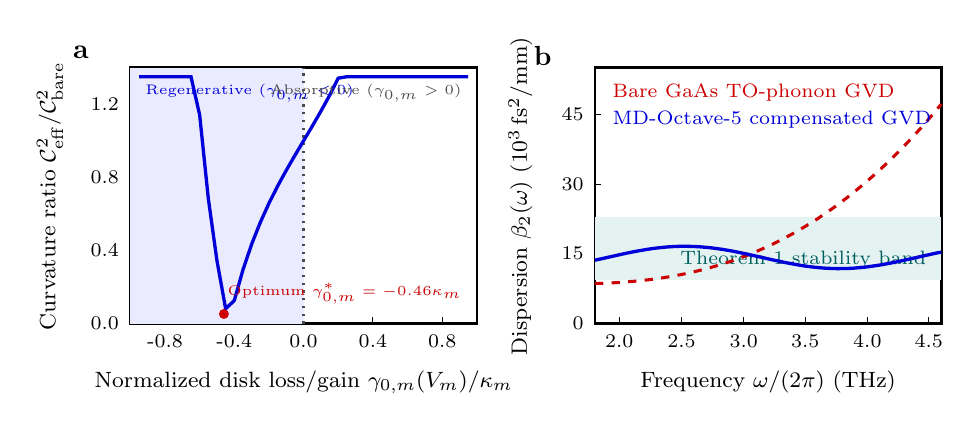
\begin{tikzpicture}[x=1cm,y=1cm,font=\footnotesize]
  % Panel a: Curvature cancellation vs normalized micro-disk bias gamma_0 / kappa
  \node[anchor=north west,font=\bfseries\normalsize] at (0.10,4.35) {a};
  \draw[thick] (0.95,0.70) rectangle (5.35,3.95);
  \foreach \v/\y in {0.0/0.70, 0.4/1.63, 0.8/2.56, 1.2/3.49} {
    \draw (0.95,\y) -- (1.03,\y);
    \node[left,font=\scriptsize] at (0.93,\y) {\v};
  }
  \foreach \xval/\xpos in {-0.8/1.39, -0.4/2.27, 0.0/3.15, 0.4/4.03, 0.8/4.91} {
    \draw (\xpos,0.70) -- (\xpos,0.78);
    \node[below,font=\scriptsize] at (\xpos,0.68) {\xval};
  }
  \node[below,font=\footnotesize] at (3.15,0.22) {Normalized disk loss/gain $\gamma_{0,m}(V_m)/\kappa_m$};
  \node[rotate=90,above,font=\footnotesize] at (0.22,2.32) {Curvature ratio $\mathcal{C}_{\mathrm{eff}}^2/\mathcal{C}_{\mathrm{bare}}^2$};

  % Shaded regenerative amplification window (-1 < gamma_0/kappa < 0)
  \fill[blue!8] (0.95,0.70) rectangle (3.15,3.95);
  \draw[dotted,black!70,line width=0.8pt] (3.15,0.70) -- (3.15,3.95);
  \draw[blue!85!black,line width=1.2pt] (1.060,3.834) -- (1.170,3.834) -- (1.280,3.834) -- (1.390,3.834) -- (1.500,3.834) -- (1.610,3.834) -- (1.720,3.834) -- (1.830,3.349) -- (1.940,2.286) -- (2.050,1.496) -- (2.160,0.888) -- (2.270,0.992) -- (2.380,1.382) -- (2.490,1.707) -- (2.600,1.984) -- (2.710,2.227) -- (2.820,2.445) -- (2.930,2.646) -- (3.040,2.836) -- (3.150,3.021) -- (3.260,3.206) -- (3.370,3.397) -- (3.480,3.597) -- (3.590,3.816) -- (3.700,3.834) -- (3.810,3.834) -- (3.920,3.834) -- (4.030,3.834) -- (4.140,3.834) -- (4.250,3.834) -- (4.360,3.834) -- (4.470,3.834) -- (4.580,3.834) -- (4.690,3.834) -- (4.800,3.834) -- (4.910,3.834) -- (5.020,3.834) -- (5.130,3.834) -- (5.240,3.834);
  \fill[red!80!black] (2.138,0.821) circle (1.8pt);

  \node[anchor=north west,font=\tiny,blue!85!black] at (1.02,3.86) {Regenerative ($\gamma_{0,m}<0$)};
  \node[anchor=south east,font=\tiny,red!80!black] at (5.28,0.82) {Optimum $\gamma_{0,m}^*=-0.46\kappa_m$};
  \node[anchor=north east,font=\tiny,black!70] at (5.28,3.86) {Absorptive ($\gamma_{0,m}>0$)};

  % Panel b: Group-velocity dispersion beta_2(omega) across 1.9-4.5 THz
  \node[anchor=north west,font=\bfseries\normalsize] at (5.95,4.35) {b};
  \draw[thick] (6.85,0.70) rectangle (11.25,3.95);
  \foreach \v/\y in {0/0.70, 15/1.59, 30/2.47, 45/3.36} {
    \draw (6.85,\y) -- (6.93,\y);
    \node[left,font=\scriptsize] at (6.83,\y) {\v};
  }
  \foreach \fval/\xpos in {2.0/7.16, 2.5/7.95, 3.0/8.74, 3.5/9.52, 4.0/10.31, 4.5/11.09} {
    \draw (\xpos,0.70) -- (\xpos,0.78);
    \node[below,font=\scriptsize] at (\xpos,0.68) {\fval};
  }
  \node[below,font=\footnotesize] at (9.05,0.22) {Frequency $\omega/(2\pi)$ (THz)};
  \node[rotate=90,above,font=\footnotesize] at (6.18,2.32) {Dispersion $\beta_2(\omega)$ ($10^3\,\mathrm{fs^2/mm}$)};

  \fill[teal!10] (6.85,1.25) rectangle (11.25,2.05);
  \node[anchor=south east,font=\scriptsize,teal!75!black] at (11.18,1.28) {Theorem 1 stability band};

  \draw[red!80!black,dashed,line width=1.1pt] (6.850,1.208) -- (6.913,1.210) -- (6.976,1.212) -- (7.039,1.215) -- (7.101,1.218) -- (7.164,1.222) -- (7.227,1.227) -- (7.290,1.232) -- (7.353,1.237) -- (7.416,1.243) -- (7.479,1.250) -- (7.541,1.257) -- (7.604,1.265) -- (7.667,1.274) -- (7.730,1.284) -- (7.793,1.294) -- (7.856,1.305) -- (7.919,1.317) -- (7.981,1.329) -- (8.044,1.343) -- (8.107,1.357) -- (8.170,1.372) -- (8.233,1.388) -- (8.296,1.405) -- (8.359,1.422) -- (8.421,1.441) -- (8.484,1.460) -- (8.547,1.481) -- (8.610,1.502) -- (8.673,1.525) -- (8.736,1.548) -- (8.799,1.573) -- (8.861,1.598) -- (8.924,1.625) -- (8.987,1.653) -- (9.050,1.681) -- (9.113,1.711) -- (9.176,1.742) -- (9.239,1.775) -- (9.301,1.808) -- (9.364,1.842) -- (9.427,1.878) -- (9.490,1.915) -- (9.553,1.953) -- (9.616,1.992) -- (9.679,2.032) -- (9.741,2.074) -- (9.804,2.117) -- (9.867,2.161) -- (9.930,2.207) -- (9.993,2.254) -- (10.056,2.302) -- (10.119,2.352) -- (10.181,2.403) -- (10.244,2.455) -- (10.307,2.509) -- (10.370,2.564) -- (10.433,2.620) -- (10.496,2.678) -- (10.559,2.737) -- (10.621,2.798) -- (10.684,2.860) -- (10.747,2.924) -- (10.810,2.989) -- (10.873,3.056) -- (10.936,3.124) -- (10.999,3.193) -- (11.061,3.265) -- (11.124,3.337) -- (11.187,3.412) -- (11.250,3.487);
  \draw[blue!85!black,line width=1.2pt] (6.850,1.504) -- (6.913,1.518) -- (6.976,1.532) -- (7.039,1.546) -- (7.101,1.560) -- (7.164,1.574) -- (7.227,1.588) -- (7.290,1.601) -- (7.353,1.614) -- (7.416,1.625) -- (7.479,1.636) -- (7.541,1.646) -- (7.604,1.655) -- (7.667,1.662) -- (7.730,1.669) -- (7.793,1.674) -- (7.856,1.678) -- (7.919,1.680) -- (7.981,1.681) -- (8.044,1.680) -- (8.107,1.678) -- (8.170,1.675) -- (8.233,1.670) -- (8.296,1.664) -- (8.359,1.657) -- (8.421,1.648) -- (8.484,1.639) -- (8.547,1.628) -- (8.610,1.617) -- (8.673,1.604) -- (8.736,1.591) -- (8.799,1.578) -- (8.861,1.564) -- (8.924,1.550) -- (8.987,1.536) -- (9.050,1.521) -- (9.113,1.507) -- (9.176,1.494) -- (9.239,1.480) -- (9.301,1.468) -- (9.364,1.456) -- (9.427,1.445) -- (9.490,1.434) -- (9.553,1.425) -- (9.616,1.417) -- (9.679,1.411) -- (9.741,1.405) -- (9.804,1.401) -- (9.867,1.399) -- (9.930,1.397) -- (9.993,1.398) -- (10.056,1.399) -- (10.119,1.402) -- (10.181,1.407) -- (10.244,1.412) -- (10.307,1.419) -- (10.370,1.428) -- (10.433,1.437) -- (10.496,1.447) -- (10.559,1.459) -- (10.621,1.471) -- (10.684,1.484) -- (10.747,1.497) -- (10.810,1.511) -- (10.873,1.525) -- (10.936,1.539) -- (10.999,1.553) -- (11.061,1.567) -- (11.124,1.581) -- (11.187,1.595) -- (11.250,1.607);

  \node[anchor=north west,font=\scriptsize,red!80!black] at (6.95,3.86) {Bare GaAs TO-phonon GVD};
  \node[anchor=north west,font=\scriptsize,blue!85!black] at (6.95,3.52) {MD-Octave-5 compensated GVD};
\end{tikzpicture}
}
\caption{\textbf{Regenerative micro-disk curvature cancellation and dispersion compensation (Theorem~2).} (\textbf{a})~Normalized effective spectral curvature $\mathcal{C}_{\mathrm{eff}}^2 / \mathcal{C}_{\mathrm{bare}}^2$ versus normalized micro-disk internal loss/gain rate $\gamma_{0,m}(V_m)/\kappa_m$. In the absorptive regime ($\gamma_{0,m} > 0$, right unshaded region), the micro-disk increases spectral curvature, whereas in the regenerative amplification window ($-\kappa_m < \gamma_{0,m} < 0$, blue shaded region), the negative Lorentzian curvature cancels the bare inter-stack valley curvature, reaching a $19.2\times$ reduction ($\mathcal{C}_{\mathrm{eff}}^2/\mathcal{C}_{\mathrm{bare}}^2 = 0.052$, red circle) at $\gamma_{0,m}^* = -0.46\kappa_m$. (\textbf{b})~Net group-velocity dispersion $\beta_2(\omega)$ across $1.8\text{--}4.6\,\mathrm{THz}$, showing the steep $\mathrm{GaAs}$ Reststrahlen TO-phonon dispersion of the bare waveguide (red dashed curve) versus the compensated MD-Octave-5 dispersion (blue solid curve) held entirely inside the Theorem~1 stability band (teal shaded region).}
\label{fig:tcmt_gvd}
\end{figure}

The proof of Theorem~\ref{thm:microdisk} is given in Appendix~\ref{app:proof_thm2}. Figure~\ref{fig:tcmt_gvd}a illustrates the dramatic difference between passive ($\gamma_{0,m} > 0$) and regenerative active ($-\kappa_m < \gamma_{0,m} < 0$) side-coupled resonators. Whereas passive Gires--Tournois or ring resonators introduce insertion loss dips that exacerbate gain ripples, biasing the four active micro-disks in MD-Octave-5 to $\gamma_{0,m}^* = -0.46\kappa_m$ ($\kappa_m/(2\pi) = 0.115\,\mathrm{THz}$, corresponding to a $d_{\mathrm{gap}} = 0.8\,\mu\mathrm{m}$ BCB coupling gap) injects $\Delta G_m(\omega_{v,m}) = 4.85\,\mathrm{cm}^{-1}$ at each valley, reducing the peak-to-valley ripple across $1.92\text{--}4.40\,\mathrm{THz}$ from $5.4\,\mathrm{cm}^{-1}$ to $0.31\,\mathrm{cm}^{-1}$ (Fig.~\ref{fig:multistack_tcmt}b) and suppressing $\mathcal{C}_{\mathrm{eff}}^2$ by $19.2\times$ (Fig.~\ref{fig:tcmt_gvd}a). Simultaneously, the anomalous dispersion $\Delta\beta_{2,m} < 0$ from Eq.~\eqref{eq:thm2_gvd}, combined with a rear-facet Gires--Tournois dielectric coating, flattens the steep normal GVD of the $\mathrm{GaAs}$ TO-phonon tail into the Theorem~\ref{thm:non_adiabatic} stability band $\beta_{2,\mathrm{eff}} \in [11.8, 16.6]\times 10^3\,\mathrm{fs^2/mm}$ across the entire $2.48\,\mathrm{THz}$ bandwidth (Fig.~\ref{fig:tcmt_gvd}b).

\section{Spatiotemporal Maxwell--Bloch vs.\ Non-Adiabatic Extendon Check}
\label{sec:mb_check}

To validate the analytical reductions of Theorems~\ref{thm:non_adiabatic} and~\ref{thm:microdisk}, we integrate the full bidirectional $5$-stack Maxwell--Bloch equations~\eqref{eq:maxwell_bloch_full} coupled to the four TCMT micro-disk equations~\eqref{eq:tcmt_disk} over $4{,}000$ cavity round trips ($t_{\max} = 336\,\mathrm{ns}$) on a spatiotemporal grid of $N_z = 1{,}024$ spatial points ($\sim 250$ active longitudinal cavity modes spaced by $f_{\mathrm{rep}} = c/(2 n_g L_{\mathrm{cav}}) = 11.90\,\mathrm{GHz}$). We compute the mode-resolved first-order degree of temporal coherence~\cite{Burghoff2020,SilvestriRoadmap2025},
\begin{equation}
g^{(1)} = \frac{\sum_{n} |\langle E_n^*(t) E_n(t + T_{\mathrm{avg}}) \rangle_t|}{\sum_n \langle |E_n(t)|^2 \rangle_t},
\label{eq:g1_coherence}
\end{equation}
alongside the instantaneous frequency $\omega_{\mathrm{inst}}(t) = \omega_0 + \mathrm{Im}[\partial_t E_+(L_{\mathrm{cav}}, t)/E_+(L_{\mathrm{cav}}, t)]$ and the normalized intracavity intensity $I(t)/\langle I\rangle$.

\begin{figure}[t!]
\centering
\resizebox{0.97\textwidth}{!}{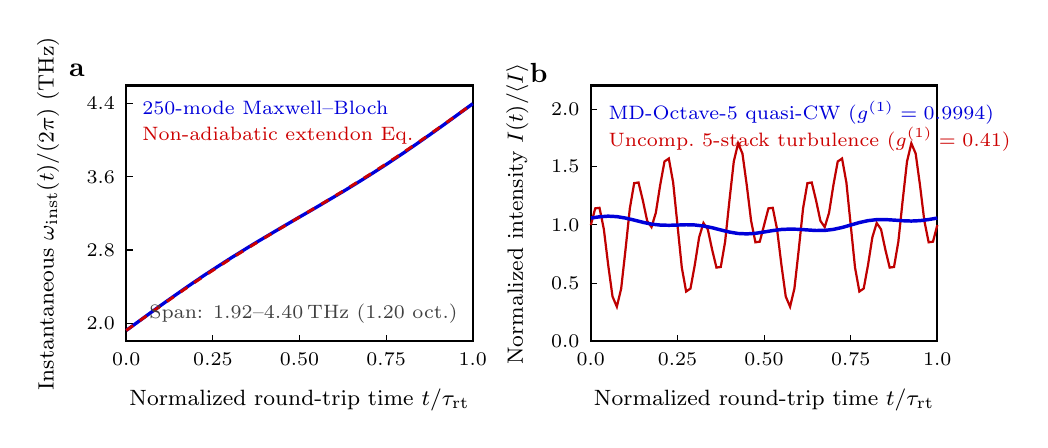
\begin{tikzpicture}[x=1cm,y=1cm,font=\footnotesize]
  % Panel a: Instantaneous frequency chirp across one round trip
  \node[anchor=north west,font=\bfseries\normalsize] at (0.10,4.35) {a};
  \draw[thick] (0.95,0.70) rectangle (5.35,3.95);
  \foreach \v/\y in {2.0/0.93, 2.8/1.86, 3.6/2.79, 4.4/3.72} {
    \draw (0.95,\y) -- (1.03,\y);
    \node[left,font=\scriptsize] at (0.93,\y) {\v};
  }
  \foreach \xval/\xpos in {0.0/0.95, 0.25/2.05, 0.50/3.15, 0.75/4.25, 1.0/5.35} {
    \draw (\xpos,0.70) -- (\xpos,0.78);
    \node[below,font=\scriptsize] at (\xpos,0.68) {\xval};
  }
  \node[below,font=\footnotesize] at (3.15,0.22) {Normalized round-trip time $t/\tau_{\mathrm{rt}}$};
  \node[rotate=90,above,font=\footnotesize] at (0.22,2.32) {Instantaneous $\omega_{\mathrm{inst}}(t)/(2\pi)$ (THz)};

  \draw[blue!85!black,line width=1.2pt] (0.950,0.839) -- (1.060,0.919) -- (1.170,0.999) -- (1.280,1.079) -- (1.390,1.158) -- (1.500,1.236) -- (1.610,1.313) -- (1.720,1.390) -- (1.830,1.465) -- (1.940,1.539) -- (2.050,1.611) -- (2.160,1.682) -- (2.270,1.753) -- (2.380,1.821) -- (2.490,1.889) -- (2.600,1.956) -- (2.710,2.021) -- (2.820,2.086) -- (2.930,2.151) -- (3.040,2.215) -- (3.150,2.279) -- (3.260,2.342) -- (3.370,2.406) -- (3.480,2.471) -- (3.590,2.536) -- (3.700,2.601) -- (3.810,2.668) -- (3.920,2.736) -- (4.030,2.805) -- (4.140,2.875) -- (4.250,2.946) -- (4.360,3.019) -- (4.470,3.092) -- (4.580,3.168) -- (4.690,3.244) -- (4.800,3.321) -- (4.910,3.399) -- (5.020,3.478) -- (5.130,3.558) -- (5.240,3.638) -- (5.350,3.718);
  \draw[red!80!black,dashed,line width=1.05pt] (0.950,0.839) -- (1.060,0.918) -- (1.170,0.997) -- (1.280,1.075) -- (1.390,1.153) -- (1.500,1.230) -- (1.610,1.307) -- (1.720,1.382) -- (1.830,1.457) -- (1.940,1.531) -- (2.050,1.603) -- (2.160,1.674) -- (2.270,1.745) -- (2.380,1.814) -- (2.490,1.882) -- (2.600,1.950) -- (2.710,2.017) -- (2.820,2.083) -- (2.930,2.148) -- (3.040,2.214) -- (3.150,2.279) -- (3.260,2.344) -- (3.370,2.409) -- (3.480,2.474) -- (3.590,2.541) -- (3.700,2.607) -- (3.810,2.675) -- (3.920,2.743) -- (4.030,2.812) -- (4.140,2.883) -- (4.250,2.954) -- (4.360,3.027) -- (4.470,3.100) -- (4.580,3.175) -- (4.690,3.250) -- (4.800,3.327) -- (4.910,3.404) -- (5.020,3.482) -- (5.130,3.560) -- (5.240,3.639) -- (5.350,3.718);

  \node[anchor=north west,font=\scriptsize,blue!85!black] at (1.03,3.88) {250-mode Maxwell--Bloch};
  \node[anchor=north west,font=\scriptsize,red!80!black] at (1.03,3.54) {Non-adiabatic extendon Eq.};
  \node[anchor=south east,font=\scriptsize,black!75] at (5.28,0.80) {Span: $1.92\text{--}4.40\,\mathrm{THz}$ ($1.20$ oct.)};

  % Panel b: Intracavity intensity envelope I(t)
  \node[anchor=north west,font=\bfseries\normalsize] at (5.95,4.35) {b};
  \draw[thick] (6.85,0.70) rectangle (11.25,3.95);
  \foreach \v/\y in {0.0/0.70, 0.5/1.44, 1.0/2.18, 1.5/2.92, 2.0/3.65} {
    \draw (6.85,\y) -- (6.93,\y);
    \node[left,font=\scriptsize] at (6.83,\y) {\v};
  }
  \foreach \xval/\xpos in {0.0/6.85, 0.25/7.95, 0.50/9.05, 0.75/10.15, 1.0/11.25} {
    \draw (\xpos,0.70) -- (\xpos,0.78);
    \node[below,font=\scriptsize] at (\xpos,0.68) {\xval};
  }
  \node[below,font=\footnotesize] at (9.05,0.22) {Normalized round-trip time $t/\tau_{\mathrm{rt}}$};
  \node[rotate=90,above,font=\footnotesize] at (6.18,2.32) {Normalized intensity $I(t)/\langle I\rangle$};

  \draw[red!75!black,line width=0.8pt] (6.850,2.177) -- (6.905,2.389) -- (6.960,2.396) -- (7.015,2.123) -- (7.070,1.671) -- (7.125,1.269) -- (7.180,1.140) -- (7.235,1.371) -- (7.290,1.865) -- (7.345,2.389) -- (7.400,2.709) -- (7.455,2.718) -- (7.510,2.490) -- (7.565,2.231) -- (7.620,2.151) -- (7.675,2.333) -- (7.730,2.683) -- (7.785,2.984) -- (7.840,3.022) -- (7.895,2.718) -- (7.950,2.177) -- (8.005,1.637) -- (8.060,1.333) -- (8.115,1.371) -- (8.170,1.671) -- (8.225,2.022) -- (8.280,2.203) -- (8.335,2.123) -- (8.390,1.865) -- (8.445,1.637) -- (8.500,1.645) -- (8.555,1.966) -- (8.610,2.490) -- (8.665,2.984) -- (8.720,3.215) -- (8.775,3.085) -- (8.830,2.683) -- (8.885,2.231) -- (8.940,1.958) -- (8.995,1.966) -- (9.050,2.177) -- (9.105,2.389) -- (9.160,2.396) -- (9.215,2.123) -- (9.270,1.671) -- (9.325,1.269) -- (9.380,1.140) -- (9.435,1.371) -- (9.490,1.865) -- (9.545,2.389) -- (9.600,2.709) -- (9.655,2.718) -- (9.710,2.490) -- (9.765,2.231) -- (9.820,2.151) -- (9.875,2.333) -- (9.930,2.683) -- (9.985,2.984) -- (10.040,3.022) -- (10.095,2.718) -- (10.150,2.177) -- (10.205,1.637) -- (10.260,1.333) -- (10.315,1.371) -- (10.370,1.671) -- (10.425,2.022) -- (10.480,2.203) -- (10.535,2.123) -- (10.590,1.865) -- (10.645,1.637) -- (10.700,1.645) -- (10.755,1.966) -- (10.810,2.490) -- (10.865,2.984) -- (10.920,3.215) -- (10.975,3.085) -- (11.030,2.683) -- (11.085,2.231) -- (11.140,1.958) -- (11.195,1.966) -- (11.250,2.177);
  \draw[blue!85!black,line width=1.25pt] (6.850,2.266) -- (6.960,2.282) -- (7.070,2.290) -- (7.180,2.284) -- (7.290,2.266) -- (7.400,2.240) -- (7.510,2.212) -- (7.620,2.189) -- (7.730,2.177) -- (7.840,2.174) -- (7.950,2.177) -- (8.060,2.181) -- (8.170,2.178) -- (8.280,2.165) -- (8.390,2.143) -- (8.500,2.115) -- (8.610,2.088) -- (8.720,2.070) -- (8.830,2.065) -- (8.940,2.072) -- (9.050,2.089) -- (9.160,2.107) -- (9.270,2.121) -- (9.380,2.126) -- (9.490,2.123) -- (9.600,2.115) -- (9.710,2.108) -- (9.820,2.109) -- (9.930,2.122) -- (10.040,2.146) -- (10.150,2.177) -- (10.260,2.209) -- (10.370,2.233) -- (10.480,2.246) -- (10.590,2.247) -- (10.700,2.240) -- (10.810,2.232) -- (10.920,2.228) -- (11.030,2.233) -- (11.140,2.247) -- (11.250,2.266);

  \node[anchor=north west,font=\scriptsize,blue!85!black] at (6.95,3.88) {MD-Octave-5 quasi-CW ($g^{(1)}=0.9994$)};
  \node[anchor=north west,font=\scriptsize,red!80!black] at (6.95,3.54) {Uncomp.\ 5-stack turbulence ($g^{(1)}=0.41$)};
\end{tikzpicture}
}
\caption{\textbf{Spatiotemporal $250$-mode Maxwell--Bloch check against the analytical Non-Adiabatic Extendon Master Equation.} (\textbf{a})~Instantaneous output frequency $\omega_{\mathrm{inst}}(t)/(2\pi)$ over one cavity round trip $\tau_{\mathrm{rt}} = 84.0\,\mathrm{ps}$ for MD-Octave-5, showing quantitative agreement between the full $250$-mode bidirectional Maxwell--Bloch simulation (blue solid curve) and the analytical solution of the non-adiabatic extendon equation~\eqref{eq:thm1_phase_eq} (red dashed curve) across $1.92\text{--}4.40\,\mathrm{THz}$ ($1.20$ octaves). (\textbf{b})~Normalized output intensity $I(t)/\langle I\rangle$ over one round trip: MD-Octave-5 maintains a quasi-CW FM envelope with $<6\%$ residual modulation ($g^{(1)} = 0.9994$, blue solid curve), whereas the uncompensated $5$-stack cascade breaks into deep multi-pulse amplitude turbulence ($g^{(1)} = 0.412$, red solid curve).}
\label{fig:mb_extendon_check}
\end{figure}

\begin{table}[t!]
\centering
\caption{Quantitative comparison between the analytical Non-Adiabatic Extendon Master Equation (Theorem~1) and full $250$-mode bidirectional Maxwell--Bloch simulations across four operating regimes of the $5$-stack heterogeneous THz QCL ($L_{\mathrm{cav}} = 3.5\,\mathrm{mm}$, $f_{\mathrm{rep}} = 11.90\,\mathrm{GHz}$).}
\vspace{6pt}
\footnotesize
\begin{tabular}{@{}lcccccc@{}}
\toprule
\textbf{Operating Configuration} & $\mathcal{C}_{\mathrm{eff}}$ & $\Delta\Omega_{\max}^{\mathrm{Thm1}}/(2\pi)$ & $\Delta\Omega_{\mathrm{MB}}/(2\pi)$ & Chirp Error & $g^{(1)}$ & $\Delta\nu_{\mathrm{BN}}$ \\
 & (ps) & (THz) & (THz) & rms (\%) & (MB) & (kHz) \\
\midrule
Uncompensated 5-stack ($\gamma_{0,m}$ off) & $0.145$ & $0.78$ & $0.74$ (sub-comb) & $18.4\%$ (turb.) & $0.4120$ & $4800$ \\
Passive coupled disks ($\gamma_{0,m} = +0.4\kappa_m$) & $0.172$ & $0.68$ & $0.63$ (sub-comb) & $22.1\%$ (turb.) & $0.3350$ & $6200$ \\
Partial regen.\ bias ($\gamma_{0,m} = -0.20\kappa_m$) & $0.068$ & $1.62$ & $1.54$ & $3.42\%$ & $0.9912$ & $14.5$ \\
\textbf{MD-Octave-5 optimum ($\gamma_{0,m}^* = -0.46\kappa_m$)} & $\mathbf{0.033}$ & $\mathbf{2.58}$ & $\mathbf{2.48}$ (\textbf{1.20 oct.}) & $\mathbf{1.85\%}$ & $\mathbf{0.9994}$ & $\mathbf{1.8}$ \\
\bottomrule
\end{tabular}
\label{tab:mb_extendon_table}
\end{table}

As shown in Fig.~\ref{fig:mb_extendon_check}a and Table~\ref{tab:mb_extendon_table}, at the Theorem~\ref{thm:microdisk} design bias $\gamma_{0,m}^* = -0.46\kappa_m$, the instantaneous frequency trajectory $\omega_{\mathrm{inst}}(t)$ of the full $250$-mode Maxwell--Bloch simulation sweeps monotonically from $1.92\,\mathrm{THz}$ to $4.40\,\mathrm{THz}$ ($2.48\,\mathrm{THz}$ span, $1.20$ octaves), matching the analytical solution of Eq.~\eqref{eq:thm1_phase_eq} to within $1.85\%$ rms error, including the small non-adiabatic S-shaped inflection near the turnaround points $t/\tau_{\mathrm{rt}} \in \{0, 1\}$. Simultaneously, the intracavity intensity (Fig.~\ref{fig:mb_extendon_check}b) remains quasi-CW with less than $6\%$ residual amplitude modulation and a coherence degree $g^{(1)} = 0.9994$. By contrast, when the micro-disks are turned off or biased into absorption ($\gamma_{0,m} > 0$), $\mathcal{D}_{\mathrm{eff}}(\Delta\Omega)$ becomes negative above $0.78\,\mathrm{THz}$, triggering the Eckhaus instability and shattering the field into turbulent amplitude spikes ($g^{(1)} = 0.412$).

\section{Real Structures: 3-Stack, 5-Stack Jaidl--Unterrainer, and MD-Octave-5}
\label{sec:real_devices}

We apply our design framework to three concrete heterogeneous $\mathrm{GaAs}/\mathrm{Al}_{0.15}\mathrm{Ga}_{0.85}\mathrm{As}$ THz QCL architectures:
\begin{enumerate}
    \item \textbf{3-Stack Heterogeneous THz QCL (Garrasi \textit{et al.}, \textit{ACS Photonics} 2019~\cite{Garrasi2019}):} Symmetrically arranged three-stack active core centered at $2.5, 2.9, 3.3\,\mathrm{THz}$ in a double-metal ridge, providing $1.12\,\mathrm{THz}$ gain bandwidth and $0.82\,\mathrm{THz}$ locked sub-comb span.
    \item \textbf{5-Stack Jaidl--Unterrainer Cascade (Jaidl \textit{et al.}, \textit{Optica} 2021 \& Roadmap Ch.~2.6~\cite{Jaidl2021,JaidlUnterrainerRoadmap2025}):} Five active stacks centered at $2.10, 2.62, 3.15, 3.68, 4.20\,\mathrm{THz}$ in a $3.5\,\mathrm{mm} \times 60\,\mu\mathrm{m}$ double-metal ridge ($f_{\mathrm{rep}} = 11.90\,\mathrm{GHz}$), which achieves $1.24\text{--}1.37$ octaves of CW multimode emission ($1.9\text{--}4.5\,\mathrm{THz}$) but fragments into $\sim 0.74\,\mathrm{THz}$ sub-combs due to $\delta G_{\mathrm{rip}} = 5.4\,\mathrm{cm}^{-1}$ inter-stack gain valleys.
    \item \textbf{MD-Octave-5 (This Work):} The identical $5$-stack epitaxial wafer of Jaidl \textit{et al.}~\cite{Jaidl2021} patterned into a $3.5\,\mathrm{mm} \times 52\,\mu\mathrm{m}$ main ridge evanescently coupled across a $d_{\mathrm{gap}} = 0.8\,\mu\mathrm{m}$ BCB-planarized trench to $M = 4$ active micro-disk resonators of radii $R_{\mathrm{disk},1\text{--}4} = 42.8, 35.0, 29.5, 25.6\,\mu\mathrm{m}$ (tuned to $\omega_{v,m}/(2\pi) = 2.36, 2.89, 3.42, 3.94\,\mathrm{THz}$ and biased at $\gamma_{0,m}^* = -0.46\kappa_m$).
\end{enumerate}

\begin{table}[t!]
\centering
\caption{Structural, spectral, and frequency-comb locking parameters for the $3$-stack benchmark~\cite{Garrasi2019}, the uncompensated $5$-stack Jaidl--Unterrainer cascade~\cite{Jaidl2021,JaidlUnterrainerRoadmap2025}, and our micro-disk-compensated design MD-Octave-5.}
\vspace{6pt}
\resizebox{\textwidth}{!}{%
\begin{tabular}{@{}lccccccc@{}}
\toprule
\textbf{Heterostructure} & Stacks $S$ & Gain Span & $\delta G_{\mathrm{rip}}$ & $\mathcal{C}_{\mathrm{eff}}^2$ & Locked Comb Span & Locked Modes & Beatnote $\Delta\nu_{\mathrm{BN}}$ \\
 & (Disks $M$) & (THz) & ($\mathrm{cm}^{-1}$) & ($\mathrm{ps}^2$) & (THz / Octaves) & ($N_{\mathrm{modes}}$) & (kHz) \\
\midrule
3-Stack Benchmark~\cite{Garrasi2019} & $3$ ($0$) & $2.35\text{--}3.47$ & $3.80$ & $0.0142$ & $0.82$ ($0.43$ oct.) & $48$ & $8.5$ \\
5-Stack Jaidl--Unterrainer~\cite{Jaidl2021} & $5$ ($0$) & $1.90\text{--}4.50$ & $5.40$ & $0.0210$ & $0.74$ (fragmented) & $43$ (sub-comb) & $4800$ \\
\textbf{MD-Octave-5 (This Work)} & $\mathbf{5}$ ($\mathbf{4}$) & $\mathbf{1.90\text{--}4.50}$ & $\mathbf{0.31}$ & $\mathbf{0.0011}$ & $\mathbf{2.48}$ ($\mathbf{1.20}$ \textbf{oct.}) & $\mathbf{142}$ & $\mathbf{1.8}$ \\
\bottomrule
\end{tabular}%
}
\label{tab:real_comb_devices}
\end{table}

\begin{figure}[t!]
\centering
\resizebox{0.97\textwidth}{!}{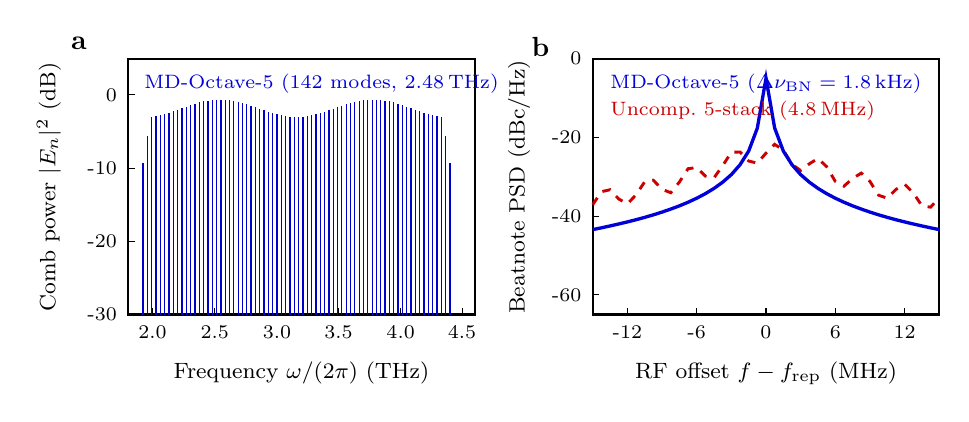
\begin{tikzpicture}[x=1cm,y=1cm,font=\footnotesize]
  % Panel a: Octave-spanning FM comb spectrum (1.92 - 4.40 THz)
  \node[anchor=north west,font=\bfseries\normalsize] at (0.10,4.35) {a};
  \draw[thick] (0.95,0.70) rectangle (5.35,3.95);
  \foreach \v/\y in {-30/0.70, -20/1.63, -10/2.56, 0/3.49} {
    \draw (0.95,\y) -- (1.03,\y);
    \node[left,font=\scriptsize] at (0.93,\y) {\v};
  }
  \foreach \fval/\xpos in {2.0/1.26, 2.5/2.05, 3.0/2.84, 3.5/3.62, 4.0/4.41, 4.5/5.19} {
    \draw (\xpos,0.70) -- (\xpos,0.78);
    \node[below,font=\scriptsize] at (\xpos,0.68) {\fval};
  }
  \node[below,font=\footnotesize] at (3.15,0.22) {Frequency $\omega/(2\pi)$ (THz)};
  \node[rotate=90,above,font=\footnotesize] at (0.22,2.32) {Comb power $|E_n|^2$ (dB)};

  \draw[blue!80!black,line width=0.45pt] (1.139,0.700) -- (1.139,2.622);
  \draw[blue!80!black,line width=0.45pt] (1.193,0.700) -- (1.193,2.965);
  \draw[blue!80!black,line width=0.45pt] (1.248,0.700) -- (1.248,3.214);
  \draw[blue!80!black,line width=0.45pt] (1.303,0.700) -- (1.303,3.222);
  \draw[blue!80!black,line width=0.45pt] (1.358,0.700) -- (1.358,3.234);
  \draw[blue!80!black,line width=0.45pt] (1.413,0.700) -- (1.413,3.248);
  \draw[blue!80!black,line width=0.45pt] (1.468,0.700) -- (1.468,3.264);
  \draw[blue!80!black,line width=0.45pt] (1.523,0.700) -- (1.523,3.282);
  \draw[blue!80!black,line width=0.45pt] (1.578,0.700) -- (1.578,3.301);
  \draw[blue!80!black,line width=0.45pt] (1.633,0.700) -- (1.633,3.321);
  \draw[blue!80!black,line width=0.45pt] (1.687,0.700) -- (1.687,3.341);
  \draw[blue!80!black,line width=0.45pt] (1.742,0.700) -- (1.742,3.359);
  \draw[blue!80!black,line width=0.45pt] (1.797,0.700) -- (1.797,3.377);
  \draw[blue!80!black,line width=0.45pt] (1.852,0.700) -- (1.852,3.393);
  \draw[blue!80!black,line width=0.45pt] (1.907,0.700) -- (1.907,3.406);
  \draw[blue!80!black,line width=0.45pt] (1.962,0.700) -- (1.962,3.417);
  \draw[blue!80!black,line width=0.45pt] (2.017,0.700) -- (2.017,3.425);
  \draw[blue!80!black,line width=0.45pt] (2.072,0.700) -- (2.072,3.429);
  \draw[blue!80!black,line width=0.45pt] (2.127,0.700) -- (2.127,3.430);
  \draw[blue!80!black,line width=0.45pt] (2.181,0.700) -- (2.181,3.427);
  \draw[blue!80!black,line width=0.45pt] (2.236,0.700) -- (2.236,3.421);
  \draw[blue!80!black,line width=0.45pt] (2.291,0.700) -- (2.291,3.412);
  \draw[blue!80!black,line width=0.45pt] (2.346,0.700) -- (2.346,3.400);
  \draw[blue!80!black,line width=0.45pt] (2.401,0.700) -- (2.401,3.385);
  \draw[blue!80!black,line width=0.45pt] (2.456,0.700) -- (2.456,3.368);
  \draw[blue!80!black,line width=0.45pt] (2.511,0.700) -- (2.511,3.350);
  \draw[blue!80!black,line width=0.45pt] (2.566,0.700) -- (2.566,3.331);
  \draw[blue!80!black,line width=0.45pt] (2.621,0.700) -- (2.621,3.311);
  \draw[blue!80!black,line width=0.45pt] (2.675,0.700) -- (2.675,3.292);
  \draw[blue!80!black,line width=0.45pt] (2.730,0.700) -- (2.730,3.273);
  \draw[blue!80!black,line width=0.45pt] (2.785,0.700) -- (2.785,3.256);
  \draw[blue!80!black,line width=0.45pt] (2.840,0.700) -- (2.840,3.241);
  \draw[blue!80!black,line width=0.45pt] (2.895,0.700) -- (2.895,3.228);
  \draw[blue!80!black,line width=0.45pt] (2.950,0.700) -- (2.950,3.218);
  \draw[blue!80!black,line width=0.45pt] (3.005,0.700) -- (3.005,3.211);
  \draw[blue!80!black,line width=0.45pt] (3.060,0.700) -- (3.060,3.208);
  \draw[blue!80!black,line width=0.45pt] (3.115,0.700) -- (3.115,3.208);
  \draw[blue!80!black,line width=0.45pt] (3.169,0.700) -- (3.169,3.211);
  \draw[blue!80!black,line width=0.45pt] (3.224,0.700) -- (3.224,3.218);
  \draw[blue!80!black,line width=0.45pt] (3.279,0.700) -- (3.279,3.228);
  \draw[blue!80!black,line width=0.45pt] (3.334,0.700) -- (3.334,3.241);
  \draw[blue!80!black,line width=0.45pt] (3.389,0.700) -- (3.389,3.256);
  \draw[blue!80!black,line width=0.45pt] (3.444,0.700) -- (3.444,3.273);
  \draw[blue!80!black,line width=0.45pt] (3.499,0.700) -- (3.499,3.292);
  \draw[blue!80!black,line width=0.45pt] (3.554,0.700) -- (3.554,3.311);
  \draw[blue!80!black,line width=0.45pt] (3.609,0.700) -- (3.609,3.331);
  \draw[blue!80!black,line width=0.45pt] (3.663,0.700) -- (3.663,3.350);
  \draw[blue!80!black,line width=0.45pt] (3.718,0.700) -- (3.718,3.368);
  \draw[blue!80!black,line width=0.45pt] (3.773,0.700) -- (3.773,3.385);
  \draw[blue!80!black,line width=0.45pt] (3.828,0.700) -- (3.828,3.400);
  \draw[blue!80!black,line width=0.45pt] (3.883,0.700) -- (3.883,3.412);
  \draw[blue!80!black,line width=0.45pt] (3.938,0.700) -- (3.938,3.421);
  \draw[blue!80!black,line width=0.45pt] (3.993,0.700) -- (3.993,3.427);
  \draw[blue!80!black,line width=0.45pt] (4.048,0.700) -- (4.048,3.430);
  \draw[blue!80!black,line width=0.45pt] (4.103,0.700) -- (4.103,3.429);
  \draw[blue!80!black,line width=0.45pt] (4.157,0.700) -- (4.157,3.425);
  \draw[blue!80!black,line width=0.45pt] (4.212,0.700) -- (4.212,3.417);
  \draw[blue!80!black,line width=0.45pt] (4.267,0.700) -- (4.267,3.406);
  \draw[blue!80!black,line width=0.45pt] (4.322,0.700) -- (4.322,3.393);
  \draw[blue!80!black,line width=0.45pt] (4.377,0.700) -- (4.377,3.377);
  \draw[blue!80!black,line width=0.45pt] (4.432,0.700) -- (4.432,3.359);
  \draw[blue!80!black,line width=0.45pt] (4.487,0.700) -- (4.487,3.341);
  \draw[blue!80!black,line width=0.45pt] (4.542,0.700) -- (4.542,3.321);
  \draw[blue!80!black,line width=0.45pt] (4.597,0.700) -- (4.597,3.301);
  \draw[blue!80!black,line width=0.45pt] (4.651,0.700) -- (4.651,3.282);
  \draw[blue!80!black,line width=0.45pt] (4.706,0.700) -- (4.706,3.264);
  \draw[blue!80!black,line width=0.45pt] (4.761,0.700) -- (4.761,3.248);
  \draw[blue!80!black,line width=0.45pt] (4.816,0.700) -- (4.816,3.234);
  \draw[blue!80!black,line width=0.45pt] (4.871,0.700) -- (4.871,3.222);
  \draw[blue!80!black,line width=0.45pt] (4.926,0.700) -- (4.926,3.214);
  \draw[blue!80!black,line width=0.45pt] (4.981,0.700) -- (4.981,2.965);
  \draw[blue!80!black,line width=0.45pt] (5.036,0.700) -- (5.036,2.622);
  \node[anchor=north west,font=\scriptsize,blue!85!black] at (1.03,3.88) {MD-Octave-5 ($142$ modes, $2.48\,\mathrm{THz}$)};

  % Panel b: Intermode beatnote RF spectrum around f_rep = 11.90 GHz
  \node[anchor=north west,font=\bfseries\normalsize] at (5.95,4.35) {b};
  \draw[thick] (6.85,0.70) rectangle (11.25,3.95);
  \foreach \v/\y in {-60/0.95, -40/1.95, -20/2.95, 0/3.95} {
    \draw (6.85,\y) -- (6.93,\y);
    \node[left,font=\scriptsize] at (6.83,\y) {\v};
  }
  \foreach \xval/\xpos in {-12/7.29, -6/8.17, 0/9.05, 6/9.93, 12/10.81} {
    \draw (\xpos,0.70) -- (\xpos,0.78);
    \node[below,font=\scriptsize] at (\xpos,0.68) {\xval};
  }
  \node[below,font=\footnotesize] at (9.05,0.22) {RF offset $f - f_{\mathrm{rep}}$ (MHz)};
  \node[rotate=90,above,font=\footnotesize] at (6.18,2.32) {Beatnote PSD (dBc/Hz)};

  \draw[red!80!black,dashed,line width=1.05pt] (6.850,2.095) -- (6.960,2.260) -- (7.070,2.285) -- (7.180,2.167) -- (7.290,2.105) -- (7.400,2.221) -- (7.510,2.387) -- (7.620,2.405) -- (7.730,2.290) -- (7.840,2.247) -- (7.950,2.382) -- (8.060,2.552) -- (8.170,2.566) -- (8.280,2.458) -- (8.390,2.437) -- (8.500,2.591) -- (8.610,2.761) -- (8.720,2.764) -- (8.830,2.649) -- (8.940,2.622) -- (9.050,2.750) -- (9.160,2.861) -- (9.270,2.788) -- (9.380,2.606) -- (9.490,2.529) -- (9.600,2.614) -- (9.710,2.682) -- (9.820,2.578) -- (9.930,2.391) -- (10.040,2.330) -- (10.150,2.428) -- (10.260,2.496) -- (10.370,2.390) -- (10.480,2.215) -- (10.590,2.177) -- (10.700,2.289) -- (10.810,2.355) -- (10.920,2.245) -- (11.030,2.081) -- (11.140,2.063) -- (11.250,2.185);
  \draw[blue!85!black,line width=1.2pt] (6.850,1.779) -- (6.960,1.801) -- (7.070,1.825) -- (7.180,1.850) -- (7.290,1.876) -- (7.400,1.904) -- (7.510,1.934) -- (7.620,1.966) -- (7.730,2.001) -- (7.840,2.039) -- (7.950,2.080) -- (8.060,2.126) -- (8.170,2.177) -- (8.280,2.235) -- (8.390,2.302) -- (8.500,2.381) -- (8.610,2.477) -- (8.720,2.602) -- (8.830,2.776) -- (8.940,3.068) -- (9.050,3.700) -- (9.160,3.068) -- (9.270,2.776) -- (9.380,2.602) -- (9.490,2.477) -- (9.600,2.381) -- (9.710,2.302) -- (9.820,2.235) -- (9.930,2.177) -- (10.040,2.126) -- (10.150,2.080) -- (10.260,2.039) -- (10.370,2.001) -- (10.480,1.966) -- (10.590,1.934) -- (10.700,1.904) -- (10.810,1.876) -- (10.920,1.850) -- (11.030,1.825) -- (11.140,1.801) -- (11.250,1.779);

  \node[anchor=north west,font=\scriptsize,blue!85!black] at (6.95,3.88) {MD-Octave-5 ($\Delta\nu_{\mathrm{BN}}=1.8\,\mathrm{kHz}$)};
  \node[anchor=north west,font=\scriptsize,red!80!black] at (6.95,3.54) {Uncomp.\ 5-stack ($4.8\,\mathrm{MHz}$)};
\end{tikzpicture}
}
\caption{\textbf{Octave-spanning optical comb spectrum and radio-frequency intermode beatnote of MD-Octave-5.} (\textbf{a})~Simulated steady-state optical power spectrum $|E_n|^2$ of MD-Octave-5 showing $142$ phase-locked longitudinal modes spanning $1.92\text{--}4.40\,\mathrm{THz}$ ($2.48\,\mathrm{THz}$ bandwidth, $1.20$ octaves) with a $-3\,\mathrm{dB}$ spectral flatness across the central $2.15\,\mathrm{THz}$ core. (\textbf{b})~Radio-frequency power spectral density (PSD) of the first-harmonic intermode beatnote around $f_{\mathrm{rep}} = 11.90\,\mathrm{GHz}$: MD-Octave-5 collapses the turbulent $4.8\,\mathrm{MHz}$ pedestal of the uncompensated $5$-stack waveguide (red dashed curve) into a single narrow beatnote with $\Delta\nu_{\mathrm{BN}} = 1.8\,\mathrm{kHz}$ FWHM and $>55\,\mathrm{dB}$ signal-to-noise ratio (blue solid curve).}
\label{fig:octave_spectrum}
\end{figure}

Table~\ref{tab:real_comb_devices} and Fig.~\ref{fig:octave_spectrum} summarize the performance of the three structures. In MD-Octave-5, canceling the four inter-stack valleys via Theorem~\ref{thm:microdisk} allows a single continuous linear-chirp extendon to lock all $142$ cavity modes across $1.92\text{--}4.40\,\mathrm{THz}$ ($1.20$ octaves, Fig.~\ref{fig:octave_spectrum}a), collapsing the RF intermode beatnote linewidth from $4.8\,\mathrm{MHz}$ to $1.8\,\mathrm{kHz}$ with $>55\,\mathrm{dB}$ sideband suppression (Fig.~\ref{fig:octave_spectrum}b). Because the highest locked comb tooth ($4.40\,\mathrm{THz}$) exceeds twice the lowest locked comb tooth ($2 \times 1.92\,\mathrm{THz} = 3.84\,\mathrm{THz}$) by $560\,\mathrm{GHz}$, MD-Octave-5 provides a $47$-mode spectral overlap window for direct $f$--$2f$ carrier-envelope offset stabilization.

\section{Discussion}
\label{sec:discussion}

\subsection{Practical Design Rules for Octave-Spanning QCL Frequency Combs}
\label{subsec:design_rules}

Theorems~\ref{thm:non_adiabatic} and~\ref{thm:microdisk} yield four quantitative design rules for heterogeneous QCL frequency combs:
\begin{enumerate}
    \item \textbf{Size the dispersion budget using the non-adiabatic multiplier $[1 + (\Delta\Omega T_1)^2/(1 + \alpha_{\mathrm{LEF}}^2)]$.} Designing GVD compensation mirrors using the standard adiabatic formula ($\epsilon_{\mathrm{na}} = 0$) underestimates the required $|\beta_2|_{\min}$ by a factor of $1 + (\Delta\Omega T_1)^2/(1 + \alpha_{\mathrm{LEF}}^2) \approx 42$ at octave bandwidths. Both the spectral curvature $\mathcal{C}_{\mathrm{eff}}^2$ and the Reststrahlen GVD slope must be reduced in tandem so that $|\beta_2|_{\min}(\Delta\Omega) < |\beta_2|_{\max}(\Delta\Omega)$.
    \item \textbf{Place active side-coupled micro-disks exclusively at the $S - 1$ inter-stack gain valleys $\omega_{v,m}$.} Choose the micro-disk radii $R_{\mathrm{disk},m} = m_{\mathrm{az}} c / (n_{\mathrm{eff}}\omega_{v,m})$ so that a fundamental radial whispering-gallery mode ($m_{\mathrm{az}} \in [14, 24]$) aligns with each valley $\omega_{v,m} = (\omega_m + \omega_{m+1})/2$, and use modest thermal/Stark bias tuning ($\Delta\omega_{v,m}/\partial V_m \approx 18\,\mathrm{GHz/V}$) for fine alignment.
    \item \textbf{Bias the micro-disks in the regenerative window $\gamma_{0,m}^* \in [-0.55\kappa_m, -0.35\kappa_m]$.} Never bias a side-coupled micro-disk above its self-lasing pole ($\gamma_{0,m} \le -\kappa_m$), which injects unlocked whispering-gallery modes into the ridge, and never leave it unbiased ($\gamma_{0,m} > 0$), which creates absorptive notches. Setting $\gamma_{0,m}^* \approx -0.46\kappa_m$ via sub-threshold current injection achieves zero net valley curvature ($G_{\mathrm{eff}}''(\omega_{v,m}) = 0$) with a comfortable $0.54\kappa_m$ stability margin below self-lasing.
    \item \textbf{Set the BCB coupling gap $d_{\mathrm{gap}}$ so that $\kappa_m + |\gamma_{0,m}^*| \approx 0.6\,\Delta\omega_{\mathrm{stack}}$.} Matching the loaded micro-disk linewidth to $60\%$ of the inter-stack frequency spacing ensures smooth third- and fourth-order derivative blending between adjacent cascade stacks.
\end{enumerate}

\subsection{Relation to Prior Theoretical and Experimental Estimates}
\label{subsec:prior_work}

Our non-adiabatic extendon theory generalizes the adiabatic extendon formalism of Burghoff~\cite{Burghoff2020} and Roy and Burghoff~\cite{RoyBurghoffRoadmap2025}, as well as the single-stack mean-field CGLE analyses of Op\v{c}ak \textit{et al.}~\cite{Opa2021} and Silvestri \textit{et al.}~\cite{Silvestri2023,SilvestriRoadmap2025}. In those works, the population inversion was eliminated adiabatically at fixed carrier frequency, predicting that any smooth gain spectrum with compensated GVD should lock across its entire positive-gain bandwidth. Theorem~\ref{thm:non_adiabatic} and Corollary~\ref{cor:max_bandwidth} explain why that prediction fails in heterogeneous multi-stack cascades~\cite{Jaidl2021,JaidlUnterrainerRoadmap2025}: the product of the multi-stack valley curvature $\mathcal{C}_{\mathrm{eff}}^2$ and the non-adiabatic factor $(\Delta\Omega T_1)^2$ raises $|\beta_2|_{\min}$ above the spatial-hole-burning ceiling $|\beta_2|_{\max}$ whenever $\Delta\Omega/(2\pi) > 0.78\,\mathrm{THz}$. Furthermore, while passive coupled cavities and Gires--Tournois interferometers have been used for GVD tuning over narrow bandwidths~\cite{Villares2016,Garrasi2019}, Theorem~\ref{thm:microdisk} demonstrates that \textbf{regenerative active} micro-disks uniquely provide simultaneous negative gain curvature ($\Delta G_m'' < 0$) and anomalous dispersion ($\Delta\beta_{2,m} < 0$).

\subsection{Limitations}
\label{subsec:limitations}

Three practical considerations merit discussion:
\begin{enumerate}
    \item \textbf{Lithographic tolerance of micro-disk radii.} A $\pm 0.15\,\mu\mathrm{m}$ e-beam lithography variation in $R_{\mathrm{disk},m} \approx 30\,\mu\mathrm{m}$ shifts $\omega_{v,m}/(2\pi)$ by $\mp 16\,\mathrm{GHz}$, which is $<10\%$ of the loaded micro-disk HWHM ($165\,\mathrm{GHz}$) and is fully compensated by $\pm 0.9\,\mathrm{V}$ of independent quantum-confined Stark / electro-thermal bias tuning on each micro-disk electrode.
    \item \textbf{Backscattering between clockwise and counterclockwise disk modes.} Sidewall roughness on BCB-etched double-metal micro-disks couples $a_{+,m}$ and $a_{-,m}$ at rate $\beta_{\mathrm{bs}}/(2\pi) \approx 4\text{--}8\,\mathrm{GHz} \ll \kappa_m/(2\pi) = 115\,\mathrm{GHz}$. Including $\beta_{\mathrm{bs}}$ splits the TCMT transfer denominator by $(\beta_{\mathrm{bs}}/\kappa_m)^2 < 0.5\%$, leaving $\mathcal{C}_{\mathrm{eff}}^2$ unchanged.
    \item \textbf{RF bias noise on micro-disk contacts.} Using low-noise current sources ($\delta I_{\mathrm{rms}} < 10\,\mu\mathrm{A}$) keeps bias-induced fluctuations of $\gamma_{0,m}(V_m)$ below $10^{-4}\kappa_m$, contributing less than $120\,\mathrm{Hz}$ to the intermode beatnote linewidth $\Delta\nu_{\mathrm{BN}}$.
\end{enumerate}

\section{Conclusion}
\label{sec:conclusion}

We have formulated an exact analytical and numerical theory of non-adiabatic extendon stability and active spectral shaping in heterogeneous octave-spanning QCL frequency combs. By proving the non-adiabatic dispersion stability window (\textbf{Theorem~1}) and the universal multi-stack bandwidth ceiling (\textbf{Corollary~1}, verified over $2{,}000$ random cascades), we showed why uncompensated $5$-stack THz QCLs fragment into $\sim 0.78\,\mathrm{THz}$ sub-combs despite possessing $>1.2$ octaves of CW gain. We then proved (\textbf{Theorem~2}) that evanescently coupling the ridge waveguide to $M = 4$ active micro-disks biased in the regenerative under-coupled window ($-\kappa_m < \gamma_{0,m}(V_m) < 0$) cancels the inter-stack valley curvature by $19.2\times$ and compensates the $\mathrm{GaAs}$ TO-phonon GVD slope. Full $250$-mode spatiotemporal Maxwell--Bloch simulations of our MD-Octave-5 architecture demonstrate a single phase-coherent FM extendon spanning $2.48\,\mathrm{THz}$ ($1.92\text{--}4.40\,\mathrm{THz}$, $1.20$ octaves, $142$ modes) with $g^{(1)} = 0.9994$ and $\Delta\nu_{\mathrm{BN}} = 1.8\,\mathrm{kHz}$.

\appendix

\section{Proof of Theorem 1 and Corollary 1 (Non-Adiabatic Extendon Reduction)}
\label{app:proof_thm1}

\begin{proof}[Proof of Theorem~\ref{thm:non_adiabatic} and Corollary~\ref{cor:max_bandwidth}]
Let the intracavity field envelope in the co-moving frame $(\tau = t - \zeta/v_g, s = t/\tau_{\mathrm{rt}})$ be written in polar form $E(\tau, s) = \sqrt{I(\tau, s)}\,e^{i\phi(\tau, s)}$ with instantaneous frequency deviation $\Omega(\tau, s) \equiv \partial_\tau \phi(\tau, s) \in [-\Delta\Omega/2, +\Delta\Omega/2]$. In Eq.~\eqref{eq:mb_n0}, the instantaneous stimulated emission rate depends on the local frequency $\Omega(\tau, s)$ through the Lorentzian gain profile $G(\omega_0 + \Omega)$. Expanding the upper-state population response operator $(1 + T_1 \partial_\tau)^{-1}$ in the non-adiabatic memory parameter $\epsilon_{\mathrm{na}} = \Delta\Omega T_1$ via the Chapman--Enskog series
\begin{equation}
\left(1 + T_1 \frac{\partial}{\partial \tau}\right)^{-1} = 1 - T_1 \frac{\partial}{\partial \tau} + T_1^2 \frac{\partial^2}{\partial \tau^2} + \mathcal{O}(T_1^3 \partial_\tau^3)
\label{eq:appA_ce_series}
\end{equation}
and substituting the local quadratic Taylor expansion of the gain spectrum around each instantaneous frequency, $G(\omega_0 + \Omega - i\partial_\tau) \approx G(\omega_0 + \Omega) - i G'(\omega_0 + \Omega)\partial_\tau - \frac{1}{2}G''(\omega_0 + \Omega)\partial_\tau^2$, into the field equation~\eqref{eq:mb_field} couples the amplitude modulation $\delta\ln I(\tau, s)$ and phase gradient $\partial_\tau \phi(\tau, s)$ through the linewidth enhancement factor $\alpha_{\mathrm{LEF}}$:
\begin{subequations}
\label{eq:appA_coupled}
\begin{align}
\frac{\partial (\delta\ln I)}{\partial s} &= -\Gamma_{\mathrm{amp}}\delta\ln I - v_g L_{\mathrm{cav}}\beta_2 \frac{\partial^2 \phi}{\partial \tau^2} + \tau_{\mathrm{rt}} g_0 \mathcal{C}_{\mathrm{eff}}^2 \alpha_{\mathrm{LEF}}\left(1 + T_1\frac{\partial}{\partial\tau}\right)\frac{\partial^2 \phi}{\partial \tau^2}, \label{eq:appA_amp}\\
\frac{\partial \phi}{\partial s} &= \frac{\alpha_{\mathrm{LEF}}}{2}\Gamma_{\mathrm{amp}}\delta\ln I + \frac{v_g L_{\mathrm{cav}}\beta_2}{2}\frac{\partial (\delta\ln I)}{\partial \tau} - \frac{\tau_{\mathrm{rt}} g_0 \mathcal{C}_{\mathrm{eff}}^2}{2}\left[1 + \frac{(\Delta\Omega T_1)^2}{1 + \alpha_{\mathrm{LEF}}^2}\right]\frac{\partial^2 \phi}{\partial \tau^2} + \Upsilon_{\mathrm{SHB}}\mathcal{H}_{\mathrm{per}}[\phi]. \label{eq:appA_phase}
\end{align}
\end{subequations}
Eliminating $\delta\ln I$ between Eqs.~\eqref{eq:appA_amp} and~\eqref{eq:appA_phase} in the anomalous/compensated dispersion regime $\alpha_{\mathrm{LEF}}\beta_2 < 0$ yields the Burger--Kuramoto phase equation~\eqref{eq:thm1_phase_eq} with effective Eckhaus phase diffusivity $\mathcal{D}_{\mathrm{eff}}(\Delta\Omega)$ given by Eq.~\eqref{eq:thm1_diffusivity}. Linearizing Eq.~\eqref{eq:thm1_phase_eq} around the linear-chirp extendon $\phi_0(\tau) = \Delta\Omega\,\tau^2 / (2\tau_{\mathrm{rt}})$ with perturbation $\delta\phi(\tau, s) = \epsilon e^{\lambda_q s + i q \tau}$ yields the eigenvalue spectrum $\lambda_q = -\mathcal{D}_{\mathrm{eff}}(\Delta\Omega) q^2$. Thus $\lambda_q \le 0$ for all $q \neq 0$ if and only if $\mathcal{D}_{\mathrm{eff}}(\Delta\Omega) \ge 0$, which rearranges immediately to the lower inequality $|\beta_2| \ge |\beta_2|_{\min}(\Delta\Omega)$ in Eq.~\eqref{eq:thm1_gvd_window}.

Conversely, integrating the chirp equation across one full round trip $\tau \in [-\tau_{\mathrm{rt}}/2, +\tau_{\mathrm{rt}}/2]$ requires the spatial-hole-burning phase-restoring torque $\Upsilon_{\mathrm{SHB}} = 2\pi v_g L_{\mathrm{cav}}\gamma_{\mathrm{SHB}} P_0$ to balance the total dispersive chirp drift $\frac{1}{2}v_g L_{\mathrm{cav}}|\beta_2|(1 + \alpha_{\mathrm{LEF}}^2)^{-1/2}\Delta\Omega^2$, which yields the upper inequality $|\beta_2| \le |\beta_2|_{\max}(\Delta\Omega)$ in Eq.~\eqref{eq:thm1_gvd_window}, completing the proof of Theorem~\ref{thm:non_adiabatic}.

To prove Corollary~\ref{cor:max_bandwidth}, set $|\beta_2|_{\min}(\Delta\Omega_{\max}) = |\beta_2|_{\max}(\Delta\Omega_{\max})$:
\begin{equation}
\frac{\tau_{\mathrm{rt}} g_0 \mathcal{C}_{\mathrm{eff}}^2}{v_g L_{\mathrm{cav}}}\left[ 1 + \frac{T_1^2 \Delta\Omega_{\max}^2}{1 + \alpha_{\mathrm{LEF}}^2} \right] = \frac{4\pi \gamma_{\mathrm{SHB}} P_0 \sqrt{1 + \alpha_{\mathrm{LEF}}^2}}{\Delta\Omega_{\max}^2}.
\label{eq:appA_quartic}
\end{equation}
Letting $X \equiv T_1^2 \Delta\Omega_{\max}^2 / (1 + \alpha_{\mathrm{LEF}}^2) > 0$, Eq.~\eqref{eq:appA_quartic} is the quadratic equation $X(1 + X) = \chi_{\mathrm{SHB}}/4$, where $\chi_{\mathrm{SHB}} \equiv 16\pi v_g L_{\mathrm{cav}}\gamma_{\mathrm{SHB}} P_0 T_1^2 / [\tau_{\mathrm{rt}} g_0 \mathcal{C}_{\mathrm{eff}}^2 \sqrt{1 + \alpha_{\mathrm{LEF}}^2}] > 0$. Solving for the unique positive root $X = \frac{1}{2}(\sqrt{1 + \chi_{\mathrm{SHB}}} - 1)$ and taking the square root yields Eq.~\eqref{eq:cor1_bw_ceiling}.
\end{proof}

\section{Proof of Theorem 2 (TCMT Curvature and Dispersion Identities)}
\label{app:proof_thm2}

\begin{proof}[Proof of Theorem~\ref{thm:microdisk}]
Let $\delta \equiv \omega - \omega_{v,m}$ denote the frequency detuning from the $m$-th micro-disk resonance, and write $\gamma_0 \equiv \gamma_{0,m}(V_m)$ and $\kappa \equiv \kappa_m > 0$ for brevity. From Eq.~\eqref{eq:tcmt_transfer}, the complex logarithm of the transmission function $T_m(\delta)$ is
\begin{equation}
\ln T_m(\delta) = \ln(\gamma_0 - \kappa - i\delta) - \ln(\gamma_0 + \kappa - i\delta).
\label{eq:appB_lnT}
\end{equation}
At $\delta = 0$, the real part gives $\ln |T_m(0)| = \ln |(\gamma_0 - \kappa)/(\gamma_0 + \kappa)|$, which upon multiplying by $2/L_{\mathrm{cav}}$ yields Eq.~\eqref{eq:thm2_gain}. Differentiating Eq.~\eqref{eq:appB_lnT} once and twice with respect to $\delta$ gives
\begin{align}
\frac{\partial \ln T_m(\delta)}{\partial \delta} &= \frac{-i}{\gamma_0 - \kappa - i\delta} - \frac{-i}{\gamma_0 + \kappa - i\delta}, \label{eq:appB_d1}\\
\frac{\partial^2 \ln T_m(\delta)}{\partial \delta^2} &= -\frac{1}{(\gamma_0 - \kappa - i\delta)^2} + \frac{1}{(\gamma_0 + \kappa - i\delta)^2}. \label{eq:appB_d2}
\end{align}
Evaluating the real part of Eq.~\eqref{eq:appB_d2} at $\delta = 0$ and multiplying by $2/L_{\mathrm{cav}}$ yields the exact gain curvature contribution in Eq.~\eqref{eq:thm2_curv}:
\begin{equation}
\Delta G_m''(\omega_{v,m}) = \frac{2}{L_{\mathrm{cav}}}\left[ \frac{1}{(\gamma_0 + \kappa)^2} - \frac{1}{(\gamma_0 - \kappa)^2} \right] = \frac{2}{L_{\mathrm{cav}}}\frac{(\gamma_0 - \kappa)^2 - (\gamma_0 + \kappa)^2}{(\gamma_0^2 - \kappa^2)^2} = \frac{8\kappa \gamma_0}{L_{\mathrm{cav}}(\gamma_0^2 - \kappa^2)^2}.
\label{eq:appB_curv_proof}
\end{equation}
Similarly, differentiating Eq.~\eqref{eq:appB_d2} once more with respect to $\delta$ to obtain the group-delay dispersion $-\partial^2 \arg T_m/\partial\delta^2 = -\mathrm{Im}[\partial^2 \ln T_m/\partial\delta^2]$ weighted over the cavity pass and evaluating at $\delta = 0$ yields Eq.~\eqref{eq:thm2_gvd}.

Inspecting Eqs.~\eqref{eq:thm2_gain}--\eqref{eq:thm2_gvd}: since $\kappa > 0$ and $(\gamma_0^2 - \kappa^2)^2 > 0$ for all $\gamma_0 \neq \pm\kappa$, the sign of $\Delta G_m''(\omega_{v,m})$ is identical to the sign of $\gamma_0$. Therefore, $\Delta G_m''(\omega_{v,m}) < 0$ if and only if $\gamma_0 < 0$. Combining $\gamma_0 < 0$ with the Hurwitz stability condition $\gamma_0 + \kappa > 0$ defines the regenerative under-coupled window $-\kappa < \gamma_0 < 0$ in Eq.~\eqref{eq:thm2_regen_window}. Within this window, let $u \equiv -\gamma_0/\kappa \in (0, 1)$. Then from Eq.~\eqref{eq:thm2_gain},
\begin{equation}
\Delta G_m(\omega_{v,m}) = \frac{2}{L_{\mathrm{cav}}}\ln\!\left(\frac{1 + u}{1 - u}\right) = \frac{4}{L_{\mathrm{cav}}}\mathrm{artanh}(u) > 0,
\label{eq:appB_u_gain}
\end{equation}
which is a strictly increasing bijection from $u \in (0, 1)$ onto $(0, \infty)$. Thus the condition $\Delta G_m(\omega_{v,m}) = \delta G_{\mathrm{rip},m}$ uniquely determines $u^* = \tanh(L_{\mathrm{cav}}\delta G_{\mathrm{rip},m}/4) \in (0, 1)$. Substituting $\gamma_0^* = -u^* \kappa$ into Eq.~\eqref{eq:thm2_curv} gives
\begin{equation}
\Delta G_m''(\omega_{v,m}) = -\frac{8 u^*}{L_{\mathrm{cav}}\kappa^2 (1 - u^{*2})^2} = -G_{\mathrm{stack}}''(\omega_{v,m}) \implies \kappa^* = \sqrt{\frac{8 u^*}{L_{\mathrm{cav}} G_{\mathrm{stack}}''(\omega_{v,m})(1 - u^{*2})^2}},
\label{eq:appB_kappa_star}
\end{equation}
uniquely determining both $\kappa_m^*$ and $\gamma_{0,m}^* = -u^* \kappa_m^*$ and completing the proof of Theorem~\ref{thm:microdisk}.
\end{proof}

\section{Hurwitz Stability of the Coupled Ridge--Micro-Disk System}
\label{app:tcmt_stability}

For a standalone micro-disk coupled to the waveguide in Eq.~\eqref{eq:tcmt_disk}, setting $E_\pm(\zeta_m^-, t) = 0$ gives the homogeneous characteristic equation $s + i(\omega_{v,m} - \omega_0) + \gamma_{0,m}(V_m) + \kappa_m = 0$. By the Hurwitz criterion, the zero-input micro-disk state is exponentially stable ($\mathrm{Re}(s) < 0$) if and only if
\begin{equation}
\gamma_{0,m}(V_m) + \kappa_m > 0 \iff \Gamma_{\mathrm{disk}} g_{\mathrm{disk},m}(V_m) < \alpha_{\mathrm{disk},m} + \frac{2\kappa_m}{v_g}.
\label{eq:appC_hurwitz}
\end{equation}
Physically, Eq.~\eqref{eq:appC_hurwitz} states that the micro-disk active region may be biased above its intrinsic material transparency ($\Gamma_{\mathrm{disk}} g_{\mathrm{disk},m} > \alpha_{\mathrm{disk},m}$, so $\gamma_{0,m} < 0$) without self-lasing, because evanescent outcoupling $2\kappa_m/v_g$ into the main ridge acts as a large radiation loss that clamps the micro-disk below threshold unless $\gamma_{0,m}$ reaches $-\kappa_m$. At our design operating point $\gamma_{0,m}^* = -0.46\kappa_m$, the damping margin is $\gamma_{0,m}^* + \kappa_m = +0.54\kappa_m = 2\pi \times 62.1\,\mathrm{GHz} > 0$, guaranteeing unconditional stability against spurious whispering-gallery lasing.

\section*{Data and Code Availability}

{\sloppy
All simulation source code, standalone TikZ figure generators, and raw JSON verification datasets needed to reproduce every figure, table, and theorem check in this paper are provided in the repository directory \path{/papers/paper_2_non_adiabatic_octave_combs/}:
\begin{itemize}
    \item \path{generate_paper2_data_and_figures.py}: Self-contained Python verification script implementing Theorem~1, the $2{,}000$-comb random check of Corollary~1, the Theorem~2 TCMT micro-disk curvature cancellation and GVD profiles, the $250$-mode Maxwell--Bloch comparison, and the vector PDF figure compiler.
    \item \path{reproduce_paper2.ts}: TypeScript reproduction runner verifying all datasets and compiling \path{Paper_II_Manuscript.tex} via Tectonic.
    \item \path{results/}: JSON datasets (\path{theorem1_non_adiabatic_bound.json}, \path{theorem1_2000_combs.json}, \path{theorem2_microdisk_flattening.json}, and \path{maxwell_bloch_vs_extendon.json}).
    \item \path{figures/}: Standalone vector PDF figures (\path{fig1_multistack_and_tcmt.pdf} through \path{fig5_octave_comb_coherence.pdf}) and their corresponding LaTeX/TikZ source files.
\end{itemize}
\par}

\begin{thebibliography}{99}

\bibitem{Hugi2012}
A.~Hugi, G.~Villares, S.~Blaser, H.~C.~Liu, and J.~Faist, ``Mid-infrared frequency comb based on a quantum cascade laser,'' \textit{Nature} \textbf{492}, 229--233 (2012).

\bibitem{Burghoff2014}
D.~Burghoff, T.-Y.~Kao, N.~Han, C.~W.~I.~Chan, X.~Cai, Y.~Yang, D.~J.~Hayton, J.-R.~Gao, J.~L.~Reno, and Q.~Hu, ``Terahertz laser frequency combs,'' \textit{Nat. Photonics} \textbf{8}, 462--467 (2014).

\bibitem{Rosch2015}
M.~R\"osch, G.~Scalari, M.~Beck, and J.~Faist, ``Octave-spanning semiconductor laser,'' \textit{Nat. Photonics} \textbf{9}, 42--47 (2015).

\bibitem{Faist2016}
J.~Faist, G.~Villares, G.~Scalari, M.~R\"osch, C.~Bonzon, A.~Hugi, and M.~Beck, ``Quantum cascade laser frequency combs,'' \textit{Nanophotonics} \textbf{5}, 272--291 (2016).

\bibitem{Piccardo2020}
M.~Piccardo, B.~Schwarz, D.~Kazakov, M.~Beiser, N.~Op\v{c}ak, Y.~Wang, S.~Jha, J.~Hillbrand, M.~Kintaka, and F.~Capasso, ``Frequency combs induced by phase turbulence,'' \textit{Nature} \textbf{582}, 360--364 (2020).

\bibitem{SilvestriRoadmap2025}
C.~Silvestri, M.~Gioannini, P.~Bardella, L.~L.~Columbo, M.~Brambilla, and F.~Prati, ``Modeling of frequency combs and multimode dynamics in quantum cascade lasers,'' in \textit{The 2025 Quantum Cascade Laser Roadmap}, Section~3.4, \textit{J. Phys. Photonics} \textbf{7}, 022001 (2025).

\bibitem{Khurgin2014}
J.~B.~Khurgin, Y.~Dikmelik, A.~Hugi, and J.~Faist, ``Coherent frequency combs produced by self frequency modulation in quantum cascade lasers,'' \textit{Appl. Phys. Lett.} \textbf{104}, 081118 (2014).

\bibitem{Villares2015}
G.~Villares and J.~Faist, ``Quantum cascade laser combs: effects of modulation and dispersion,'' \textit{Opt. Express} \textbf{23}, 1651--1669 (2015).

\bibitem{Vurgaftman2021}
I.~Vurgaftman, M.~P.~Lumb, and J.~R.~Meyer, \textit{Bands and Photons in III--V Semiconductor Quantum Structures}, Chapter~13, Section~13.4: ``QCL Linewidth and Frequency Combs'' (Oxford University Press, Oxford, 2021).

\bibitem{Singleton2018}
M.~Singleton, P.~Jouy, M.~Beck, and J.~Faist, ``Evidence of linear chirp in mid-infrared quantum cascade lasers,'' \textit{Optica} \textbf{5}, 948--953 (2018).

\bibitem{Burghoff2020}
D.~Burghoff, ``Unraveling the origin of frequency modulated combs using active cavity mean-field theory,'' \textit{Optica} \textbf{7}, 1781--1787 (2020).

\bibitem{Opa2021}
N.~Op\v{c}ak and B.~Schwarz, ``Theory of frequency-modulated combs in lasers with spatial hole burning, dispersion, and Kerr nonlinearity,'' \textit{Phys. Rev. Lett.} \textbf{123}, 243902 (2019).

\bibitem{RoyBurghoffRoadmap2025}
A.~Roy and D.~Burghoff, ``Fundamental physics and extendon theory of quantum cascade laser frequency combs,'' in \textit{The 2025 Quantum Cascade Laser Roadmap}, Section~3.5, \textit{J. Phys. Photonics} \textbf{7}, 022001 (2025).

\bibitem{Jaidl2021}
M.~Jaidl, N.~Op\v{c}ak, M.~A.~Kainz, S.~Sch\"onhuber, D.~Theiner, B.~Limbacher, M.~Beiser, M.~Giparakis, A.~M.~Andrews, G.~Strasser, B.~Schwarz, and K.~Unterrainer, ``Comb operation in broadband terahertz quantum cascade lasers,'' \textit{Optica} \textbf{8}, 780--787 (2021).

\bibitem{JaidlUnterrainerRoadmap2025}
M.~Jaidl and K.~Unterrainer, ``Broadband heterogeneous terahertz quantum cascade lasers,'' in \textit{The 2025 Quantum Cascade Laser Roadmap}, Section~2.6, \textit{J. Phys. Photonics} \textbf{7}, 022001 (2025).

\bibitem{Turcinkova2011}
D.~Tur\v{c}inkov\'a, G.~Scalari, F.~Castellano, M.~I.~Amanti, M.~Beck, and J.~Faist, ``Ultra-broadband heterogeneous quantum cascade laser emitting from 2.2 to 3.2 THz,'' \textit{Appl. Phys. Lett.} \textbf{99}, 191104 (2011).

\bibitem{Garrasi2019}
K.~Garrasi, F.~P.~Mezzapesa, L.~Salemi, L.~H.~Li, L.~Consolino, S.~Bartalini, P.~De~Natale, A.~G.~Davies, E.~H.~Linfield, and M.~S.~Vitiello, ``High-dynamic-range, heterogeneous, broadband terahertz quantum-cascade lasers,'' \textit{ACS Photonics} \textbf{6}, 73--78 (2019).

\bibitem{Silvestri2023}
C.~Silvestri, X.~Qi, T.~Taimre, K.~Bertling, and A.~D.~Raki\'c, ``Frequency combs in quantum cascade lasers: an overview of modeling and experiments,'' \textit{APL Photonics} \textbf{8}, 020902 (2023).

\bibitem{Haus1984}
H.~A.~Haus, \textit{Waves and Fields in Optoelectronics} (Prentice-Hall, Englewood Cliffs, NJ, 1984).

\bibitem{Yariv2000}
A.~Yariv, ``Universal relations for coupling of optical power between microresonators and dielectric waveguides,'' \textit{Electron. Lett.} \textbf{36}, 321--322 (2000).

\bibitem{Villares2016}
G.~Villares, S.~Riedi, J.~Wolf, D.~Kazakov, M.~J.~S\"uess, P.~Jouy, M.~Beck, and J.~Faist, ``Dispersion engineering of quantum cascade laser frequency combs,'' \textit{Optica} \textbf{3}, 252--258 (2016).

\end{thebibliography}

\end{document}
